\documentclass[12pt,a4paper]{report}
\usepackage[utf8]{inputenc}
\usepackage[left=1.00in, right=1.00in, top=1.00in, bottom=1.00in]{geometry}
\usepackage{amsmath}
\usepackage{amssymb}
\usepackage{graphicx}
\usepackage{xcolor}
\usepackage{subfig}
\graphicspath{{images/}}
\usepackage{tikz}
\usepackage{tikz-3dplot}
\usepackage{pgfplots}
\usepackage{epstopdf}
\usepackage{float}
\usepackage{titlesec}
\usepackage{tcolorbox}
\newcommand*{\permcomb}[4][0mu]{{{}^{#3}\mkern#1#2_{#4}}}
\newcommand*{\perm}[1][-3mu]{\permcomb[#1]{P}}
\newcommand*{\comb}[1][-1mu]{\permcomb[#1]{C}}
\usepackage{lipsum}
\usepackage[framemethod=TikZ]{mdframed}
\mdfdefinestyle{MyFrame}{%
    linecolor=black,
    outerlinewidth=2pt,
    roundcorner=5pt,
    innertopmargin=\baselineskip,
    innerbottommargin=\baselineskip,
    innerrightmargin=10pt,
    innerleftmargin=10pt,
    backgroundcolor= white
}

\titleformat{\chapter}
  {\Large\bfseries} % format
  {}                % label
  {0pt}             % sep
  {\huge}
%--------------------------------------------------------------------------------------
%\title{To understand the influence of  driven solutal convection on dendrite growth. }
%\author{Apaar Shanker}
%\date{April 2015}
%--------------------------------------------------------------------------------------
\begin{document}
\begin{titlepage}
\centering
\vspace{20pt}
\Large
\bfseries
Master of Science\\
Materials Science\\
\normalfont
\Large
\vspace{10pt}
Project Report\\
\vspace{100pt}
\LARGE
\bfseries
The influence of Convection on the Evolution of Microstructure 
during Solidification\\
\normalfont
\Large
\vspace{100pt}
Submitted By:-\\
Apaar Shanker\\
(SR No. 09101)\\
\vspace{20pt}
Under the guidance of\\ 
Dr. Abhik Choudhury
\end{titlepage}

%\maketitle
\pagenumbering{roman}
\tableofcontents

%\chapter*{Acknowledgements}
\addcontentsline{toc}{chapter}{Acknowledgements}
%\begin{abstract}
%\end{abstract}

\pagenumbering{arabic}

\chapter{Synopsis}
%\setcounter{chapter}{1}
%\addcontentsline{toc}{chapter}{Synopsis}

Solidification is one of the major materials processing 
techniques, where in there is a phase transformation from a 
liquid to one or more solid phases. The process gives rise to 
a variety of microstructures - arising out of dendritic, 
eutectic, peritectic and monotectic reactions.\\
\\
It is well known that properties of a material can be linked 
to its structure at the microscopic scale. Thus, in order to 
manufacture a cast product with desired properties, it is 
essential to determine the influence of the processing parameters 
on microstructural evolution. Here, simulations of computational 
models for solidification allow for the determination of the 
useful process $\rightarrow$ structure and parameter $\rightarrow$ 
structure correlations while saving up on the time, efforts and 
material costs required in manual determination of the same.\\
\\
Solidification, a first order phase transition, involves a 
transfer of heat/mass across the interface between the solid 
and the liquid phases concomitant with diffusion in the bulk 
liquid and the solid phases. Any modeling technique describing 
this phenomenon will require, that in addition to the global 
boundary conditions controlling the heat/mass exchange, it 
self-consistently is able to integrate the transport processes 
at the moving interface with those in the bulk.\\
\\
Classically, such problems were treated with 
\textbf{\textit{Sharp-interface}} methods, wherein, separate 
transport equations are solved in the respective bulk phases, while the appropriate (\textit{Stefan-boundary}) conditions 
are imposed at the interface nodes which therefore need to be
marked after each time iteration. The method becomes cumbersome
in case of complex morphological evolution which 
is commonly encountered in most solidification reactions, where
explicit interface tracking becomes computationally expensive
and resolving sharp curvatures necessitates the use of finer
meshes.\\
\\
In this context, we resort to the 
\textbf{\textit{phase field method}} - a state-of-the art
technique, developed over the past three decades which 
obviates the need for tracking of the moving interfaces.
Succinctly, the method describes evolution equations for 
order parameters varying smoothly between the various phases,
thereby representing phase evolution. The various boundary
conditions at the moving interface are self-consistently
described in the transport equations describing
solutal/heat/momentum transport, which are defined globally. 
The transport equations are coupled with the evolution equations
for the order parameter.\\
\\
This class of methods has been applied to a variety of phase transformation reactions.
Presently, we have used the phase field method to investigate the 
\textbf{\textit{influence of convection on dendritic growth}}. There is a large 
practical interest in dendritic solidification as an overwhelming majority of 
metallic systems solidify in this manner. This is also an interesting problem 
in terms of 
understanding the mechanisms of pattern selection in non-equilibrium systems and engenders a lot of theoretical 
interest.\\
\\ 
In practical set-ups the dendritic growth is unavoidably influenced by either buoyancy driven natural convection or via forced flows(stirring) in the melt phase, causing large scale transport of mass or heat. This effect of advection due to fluid flow on the evolving dendrite's morphology, has not yet been fully understand and is of great practical importance.\\ 
\\
In the present study we have endeavored to throw some light this aspect of solidification. We have set up a phase field model to simulate dendritic growth. To this, we have coupled fluid solvers, which are based on - 
\begin{enumerate}
	\item Direct numerical simulation of the navier stokes equations.
	\item Lattice Boltzmann-BGK model
\end{enumerate} 
We thus seek to directly simulate dendritic growth in a convective regime and gauge the effect of flow on the evolving morphology of the solid phase.\\
\\
\chapter{An introduction to Dendritic Solidification}

Dendritic solidification is ubiquitous in nature and is
of great practical and theoretical importance. The 
dendritic morphology can be characterised by growth 
of primary arms along well defined crystallographic 
directions with each primary arm also giving rise to 
self-similar secondary and tertiary arms.\\
\\
Dendritic microstructures result as a destabilization 
of a planar or spherical growth front. A critical 
component giving rise to dendritic morphology, where 
the primary growth occurs along well defined 
directions, is the surface energy anisotropy.\\
\\
Physically, an understanding of dendrite morphology 
and growth would entail the knowledge of the scaling 
laws pertaining to -  dendrite tip radius, inter 
dendritic and secondary arm spacings and how they 
change as a function of the processing conditions, 
alloy composition and properties. The requirement 
for understanding the scale and variation of these 
parameters lies in the fact that macroscopic parameters 
such as tensile strength, fracture toughness etc. 
are often determined by the scale of the microstructure.\\
\\
There have been significant advances in understanding 
the physics of dendritic growth. The role of crystalline 
anisotropy in the selection of the dendrite tip radius 
and velocity is well explained by the microsolvability theory \cite{MS_theory}. 
The theory has been validated by sophisticated micro gravity 
experiments as well as phase field simulations in both two and 
three dimensions, that focused on the purely diffusive 
regime.\\
\\
On earth, however, dendritic growth is almost unavoidably influenced by buoyancy driven 
mass and energy advection in the melt phase. Melt flow introduces a new length scale in 
the problem, viz. the length of the convecting rolls, and breaks the symmetry of transport 
depending on the direction of the vector of gravity relative to the direction of growth. 
Self-organizing pattern formation in solidification begins to compete with the self-organization 
of the convection patterns. On the one hand, convective transport of solute significantly alters the 
growth conditions. On the other hand, the magnitude of convection critically depends on solute 
gradients due to growth and on the friction of the convecting liquid melt against the 
growing solid-liquid interface\cite{Stein}.


\chapter{A Phase Field Model for Solidification}

\section{The Phase Field Method}

In the phase field method the system properties are expressed using a set of phasefield variables 
that vary continuously within a bound across all the phases in the system. The thermodynamics and 
transport properties of the system are coupled with or expressed in terms of the dynamics of these 
phasefield variables.\\
\\
The time evolution of the phase field variables is given by a set of coupled partial differential 
equations, one equation for each variable. The equations are derived according to the principles of 
non-equilibrium thermodynamics.They are so chosen that the free energy of the system decreases with 
time and mass is conserved for all components. Likewise transport properties within the bulk as well as 
the interface are incorporated to be consistent with the dynamics of these phasefield variables. 
Numerical solutions of these PDE's yield the temporal evolution of the phasefield variables, which is 
a representation of the morphological evolution of the "phases" in the system.\\
\\
The application of the phase field method starts with the creation of a functional which includes the 
material properties - the surface energies of the interfaces and the thermodynamic free energies 
of the bulk phases in the system. A variational derivative of this functional with respect to any of the 
phasefield variables, gives us the dynamics vis-a-vis that variable.\\


\section{The Allen-Cahn Equation}

We need to come up with an equation that encompasses the energetics of the system. 
We can start with the energy density functional for an equilibrium state $\phi_o$ and 
add energy contributions with respect to the variation from this state. This construction, 
would write as,\\
\begin{align}
	f\left(\phi,\nabla\phi,\nabla^2\phi\right) &= 
	f_o\left(\phi\right) + \dfrac{\partial f}{\partial \phi^{'}}\delta\phi^{'} 
	+ \dfrac{\partial f}{\partial \phi^{''}}\delta\phi^{''} + \dfrac{1}{2}
	\dfrac{\partial f}{\partial^2 \phi^{'}}\left(\delta\phi^{'}\right)^2
\end{align}
The energy state of the system cannot depend on the choice of the coordinate system should be rotationally invariant. This can be guaranteed only if 
\textcolor{red}{$\dfrac{\partial f}{\partial \phi^{'}\delta \phi^{'}}$} makes zero contribution to the energy integral. 
Therefore, the simplest energy density that can be written takes the following form,
\begin{align}
f\left(\phi,\nabla \phi\right)= 
f_o\left(\phi\right) + \kappa_1\left(\nabla \phi\right)^{2} + \kappa_2\left(\nabla^2 \phi\right) 
\end{align}
The total energy of the system is a volume integral of the energy density and after some more simplification 
can be written down in the functional form as,
\begin{align}
 {\cal F} &= \int_{-\infty}^{\infty}\left(f_o\left(\phi\right) + \kappa\left(\nabla \phi\right)^{2}\right) dV
\end{align}
If we were, to compute the time-derivative of the change in the free-energy functional, 
it can be written as, 
\begin{align}
 \dfrac{\delta {\cal F}}{\delta t} &= \int_{-\infty}^{\infty} \dfrac{\delta {\cal F}}{\delta \phi}\dfrac{\partial \phi}{\partial t}dx
 \label{time_derivative_free_energy}
\end{align}
Given that $\phi$ is a non conserved variable, the simplest way to ensure that the functional is minimised in time, would be,
\begin{align}
 \dfrac{\partial \phi}{\partial t} &= -M \dfrac{\delta {\cal F}}{\delta \phi},
\end{align}
such that the time derivative of the free-energy functional now reads, 
\begin{align}
 \dfrac{\delta {\cal F}}{\delta t} &= -\int_{-\infty}^{\infty}M\left(\dfrac{\delta {\cal F}}{\delta \phi}\right)^{2}dx.
\end{align}
Clearly, here, we are minimizing the energy. However, the rate of change is zero, when the functional is at an extremum given by $\dfrac{\delta {\cal F}}{\delta \phi} = 0$.\\
\\
The dynamical evolution for $\phi$ is then expressed as,
\begin{align}
 \dfrac{\partial \phi}{\partial t} &= -M \dfrac{\delta F}{\delta \phi}.
\end{align}
where 
$
\dfrac{\partial}{\partial t}
$
is operator for variational derivative and expands as,
\begin{align}
 \dfrac{\delta {\cal F}}{\delta \phi} &= \left(\dfrac{\partial}{\partial \phi} - 
 \nabla \cdot \dfrac{\partial}{\partial \nabla\phi} + \nabla^{2}\cdot\dfrac{\partial }{\partial \nabla^{2}\phi}\ldots\right)f  
 \label{variational_derivative}
\end{align}
Applying this, we derive,
\begin{align}
 \dfrac{\partial \phi}{\partial t} &= -M \left(\dfrac{\partial f_o}{\partial \phi} - 2\kappa\nabla^{2}\phi\right).
\end{align} 
This is the equation describing Allen-Cahn dynamics and is applicable to a large class of materials transformations, for example, evolution of grain-boundaries, order-disorder transitions, solidification etc.

\section{Modelling Alloy Solidification}

We have in the previous section derived the Allen-Cahn 
equation, where in, if the two phases have the same 
free energy, a stationary interface with a defined width 
is created. However, if we were to add a term to the energy
functional such that it tilts one of the energy levels with respect to the other, the phenomenological equation of motion, has so been constructed that the evolution of $\phi$ will be in a direction such that the phase with the higher energy will be consumed in favour of the phase with the lower energy.\\
\\
This then is an apt recipe for modelling solidification. Formally this tilting, or rather the departure from equilibrium between the two phases, can be expressed as the \textit{driving force} for phase transformation. In the case of solidification of binary isomorphous alloy, at a given under cooling, the driving force arises due to deviation of the diffusion potential from the equilibrium and results in solute rejection at the interface and expansion of the solidification front.\\
\\
    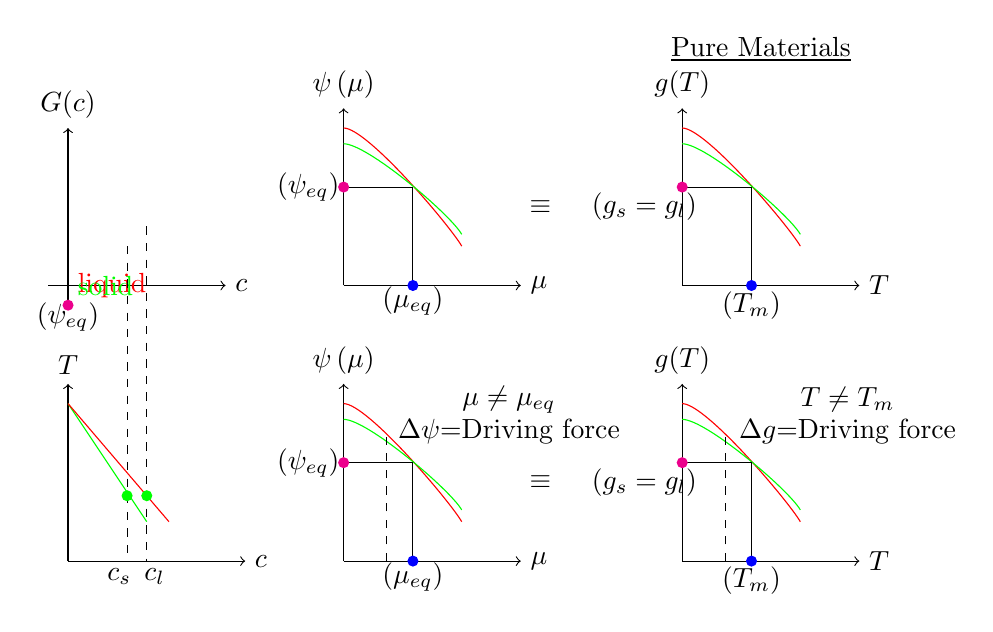
\begin{tikzpicture}[domain=0:1.75]
    %   \draw[very thin, color=gray] (0.0,1.7) grid (1.7,1.7);
    \begin{scope}
      \draw[->] (-0.25,0)--(2,0) node[right]{$c$};
      \draw[->] (0,-0.25)--(0,2) node[above]{$G(c)$};
      \draw[color=red] plot[id=x] function{((x-0.5)**2) + 0.5}
      node[right] {liquid};
      \draw[color=green] plot[id=x1] function{((x-0.25)**2) + 0.25}
      node[right] {solid};
      \draw[color=blue] plot[id=x2] function{3./4 + (x-1)};
      \fill[magenta] (0,-0.25) circle(2pt);
      \node at (0,-0.4){($\psi_{eq}$)};
    \end{scope}
    \begin{scope}[xshift=3.5cm]
    \draw[->] (0,0)--(2.25,0) node[right]{$\mu$};
    \draw[->] (0,0)--(0,2.25) node[above]{$\psi\left(\mu\right)$};
    \draw[red](0,2)..controls +(0:0.3) and +(120:0.3)..(1.5,0.5);
    \draw[green](0,1.8)..controls +(0:0.3) and +(120:0.3)..(1.5,0.65);
    \draw[] (0.88,1.25)--(0.88,0.0);
    \draw[] (0.0,1.25)--(0.88,1.25);
    \fill[blue] (0.88,0.0) circle(2pt);
    \node at (0.88,-0.2){($\mu_{eq}$)};
    \fill[magenta] (0.0,1.25) circle(2pt);
    \node at (-0.45,1.25){($\psi_{eq}$)};
    \node at (2.5,1){$\equiv$};
    \end{scope}
    \begin{scope}[xshift=7.8cm]
    \draw[->] (0,0)--(2.25,0) node[right]{$T$};
    \draw[->] (0,0)--(0,2.25) node[above]{$g(T)$};
    \draw[red](0,2)..controls +(0:0.3) and +(120:0.3)..(1.5,0.5);
    \draw[green](0,1.8)..controls +(0:0.3) and +(120:0.3)..(1.5,0.65);
    \draw[] (0.88,1.25)--(0.88,0.0);
    \draw[] (0.0,1.25)--(0.88,1.25);
    \fill[blue] (0.88,0.0) circle(2pt);
    \node at (0.88,-0.25){($T_m$)};
    \fill[magenta] (0.0,1.25) circle(2pt);
    \node at (-0.48,1.0){($g_s=g_l$)};
    \node at (1,3){\underline{Pure Materials}};
    \end{scope}
    \begin{scope}[yshift=-3.5cm]
    \draw[->] (0,0)--(2.25,0) node[right]{$c$};
    \draw[->] (0,0)--(0,2.25) node[above]{$T$};
    \draw[green] (0,2)--(1,0.5);
    \draw[red] (0,2)--(1.5/1.17,0.5);
    %  \draw[red] plot[id=x4] function{2.0-1.17*x};
    \draw[dashed] (3/4,3.5+1/2)--(3/4,0.0);
    \fill[green] (3/4,0.83) circle(2pt);
    \draw[dashed] (1,3/4+3.5)--(1,0.0);
    \node at (3/4-0.1,-0.2){$c_s$};
    \node at (1.1,-0.2){$c_l$};
    \fill[green] (1,0.83) circle(2pt);
    %  \draw[red](0,2)..controls +(0:0.3) and +(120:0.3)..(1.5,0.5);
    %  \draw[green](0,1.8)..controls +(0:0.3) and +(120:0.3)..(1.5,0.65);
    %  \draw[] (0.88,1.25)--(0.88,0.0);
    %  \draw[] (0.0,1.25)--(0.88,1.25);
    %  \fill[blue] (0.88,0.0) circle(2pt);
    %  \node at (0.88,-0.2){($\mu_{eq}$)};
    %  \fill[magenta] (0.0,1.25) circle(2pt);
    %  \node at (-0.45,1.25){($\psi_{eq}$)}; 
    \end{scope}
    \begin{scope}[xshift=3.5cm,yshift=-3.5cm]
    \draw[->] (0,0)--(2.25,0) node[right]{$\mu$};
    \draw[->] (0,0)--(0,2.25) node[above]{$\psi\left(\mu\right)$};
    \draw[red](0,2)..controls +(0:0.3) and +(120:0.3)..(1.5,0.5);
    \draw[green](0,1.8)..controls +(0:0.3) and +(120:0.3)..(1.5,0.65);
    \draw[] (0.88,1.25)--(0.88,0.0);
    \draw[] (0.0,1.25)--(0.88,1.25);
    \fill[blue] (0.88,0.0) circle(2pt);
    \node at (0.88,-0.2){($\mu_{eq}$)};
    \fill[magenta] (0.0,1.25) circle(2pt);
    \node at (-0.45,1.25){($\psi_{eq}$)};
    % \node at (2.5,2.95){\underline{Departure from equilibrium}};
    \draw[dashed](0.55,0.0)--(0.55,1.65);
    \node at (2.1,1.65){$\Delta \psi$=Driving force};
    \node at (2.1,2.05){$\mu\neq\mu_{eq}$};
    \node at (2.5,1){$\equiv$};
    \end{scope}

    \begin{scope}[xshift=7.8cm,yshift=-3.5cm]
    \draw[->] (0,0)--(2.25,0) node[right]{$T$};
    \draw[->] (0,0)--(0,2.25) node[above]{$g(T)$};
    \draw[red](0,2)..controls +(0:0.3) and +(120:0.3)..(1.5,0.5);
    \draw[green](0,1.8)..controls +(0:0.3) and +(120:0.3)..(1.5,0.65);
    \draw[] (0.88,1.25)--(0.88,0.0);
    \draw[] (0.0,1.25)--(0.88,1.25);
    \fill[blue] (0.88,0.0) circle(2pt);
    \node at (0.88,-0.25){($T_m$)};
    \fill[magenta] (0.0,1.25) circle(2pt);
    \node at (-0.48,1.0){($g_s=g_l$)};
    %  \node at (1,3){\underline{Pure Materials}};
    \node at (2.1,1.65){$\Delta g$=Driving force};
    \node at (2.1,2.05){$T\neq T_m$};
    \draw[dashed](0.55,0.0)--(0.55,1.65);
    \end{scope}
    \label{Drivingforcealloys}
    \end{tikzpicture}
   \\
  Assuming conditions of local thermodynamic equilibrium(LTE), the driving force for phase
  transformation in alloys is the difference of the grand-potentials of the solid and the liquid 
  phases (or the difference of the chemical potentials of any of the chemical entities depending 
  on whether we start from a Helmholtz free-energy density or a Gibbs-free energy 
  density in the functional).\\
\\
  In the present description, we adopt a Helmholtz free energy density. This treatment has been referenced from the work of Abhik N. Chaudhary \cite{Abhik_1}. The driving force for solidification can be described as $\Psi_l-\Psi_s$ This is analogous to the case of pure material solidification where the driving force is given by $g_l-g_s$.  
  However, while the state-variable in the case of pure material solidification is the temperature $T$, 
  it becomes the diffusion-potential $\mu$ in the case of binary alloy solidification. This analogy 
  can be well appreciated from the diagram in Fig \ref{Drivingforcealloys}.\\
  
  At equilibrium, the common-tangent construction gives the equilibrium compositions of the solid and liquid phases, which can be read from the equilibrium phase diagram. This same equilibrium can also be represented as the intersection of the grand-potential densities $\Psi\left(\mu\right)$ expressed as 
  a function of the diffusion-potentials $\mu$, where $\Psi_s\left(\mu_{eq}\right)=\Psi_l\left(\mu_{eq}\right)$, 
  in the same manner as $g_s(T_m)= g_l(T_m)$ for the case of pure materials. Away from equilibrium  $\mu\neq\mu_{eq}, \Psi_l\neq \Psi_s$, and we have a driving force for phase transition given by the difference of the grand-potential densities.\\
  \\
  Therefore, using this above analogy we can write down the driving force for phase transition for alloys purely in terms of the diffusion potential $\mu$ by performing a Taylor series expansion around equilibrium, until the 
  first order as follows, 
  \begin{align}
  \Psi_s\left(\mu\right) &= \Psi_s\left(\mu_{eq}\right) + \dfrac{\partial \Psi_s}{\partial \mu}\left(\mu-\mu_{eq}\right)\\
  \Psi_l\left(\mu\right) &= \Psi_l\left(\mu_{eq}\right) + \dfrac{\partial \Psi_l}{\partial \mu}\left(\mu-\mu_{eq}\right).
  \end{align}
  From the fig. \ref{Drivingforcealloys} it is clear that we can express the 
  grand-potential as $\Psi(\mu) = g(c(\mu)) -\mu c\left(\mu\right)$, which is the 
  essentially the \textit{Legendre transform} of $g$. Therefore, we can derive, 
  \begin{align*}
   \dfrac{\partial \Psi}{\partial \mu} &= \dfrac{\partial g}{\partial c}\dfrac{\partial c}{\partial \mu} - \mu \dfrac{\partial c}{\partial \mu} -c\\
                                       &= -c,
  \end{align*}
  where we have used $\dfrac{\partial g}{\partial c}=\mu$. Clearly, then we can write 
  the driving force for solidification $\Psi_l-\Psi_s$ as,
  
  \begin{align}
   \Psi_l-\Psi_s &= (c_s^{eq} - c_l^{eq})\left(\mu-\mu_{eq}\right),
  \end{align}  
  where we have used $\Psi_l\left(\mu_{eq}\right) = \Psi_s\left(\mu_{eq}\right)$ and $\dfrac{\partial \Psi_l}{\partial \mu}_{\mu_{eq}} = -c_l^{eq}$
  and $\dfrac{\partial \Psi_s}{\partial \mu}_{\mu_{eq}} = -c_s^{eq}$. This relation can be 
  transmitted to the evolution equation for the phase-field variable $\phi$ as,
  \begin{align}
  \dfrac{\partial \phi}{\partial t} &= -M \left(\dfrac{\partial f_o}{\partial \phi} - 2\kappa\nabla^{2}\phi\right)  
					-M\underbrace{(c_l^{eq} - c_s^{eq})\left(\mu-\mu_{eq}\right)\dfrac{\partial h\left(\phi\right)}{\partial \phi}}_{driving force}.
  \end{align}
  The evolution equation of the coupled variable $\mu$ can be derived using mass conservation. 
  Using the interpolation polynomial $h(\phi) = \phi^2\left(3 - 2\phi\right)$, which has the 
  property $h(\phi) + h(1 - \phi) = 1$, the local composition can be written as, 
  \begin{align}
   c = c_s h\left(\phi\right) + c_l (1 - h\left(\phi\right)), 
  \end{align}
Now the mass conservation equation can be written as, 
\begin{align}
 \dfrac{dc}{dt} &= \nabla\cdot\left(M\nabla\mu\right)\\
 \text{Also,}\\
	\dfrac{dc}{dt} &= \dfrac{\partial c}{\partial t} + \dfrac{\partial c}{\partial x}\dfrac{\partial x}{\partial t}
	+\dfrac{\partial c}{\partial y}\dfrac{\partial y}{\partial t}+\dfrac{\partial c}{\partial z}\dfrac{\partial z}{\partial t}
	= \dfrac{\partial c}{\partial t} + \vec{v}\cdot\nabla c\\
	\text{Thus, we have,}\\
	\dfrac{\partial c}{\partial t} &= \nabla\cdot\left(M\nabla\mu\right) - \vec{v}\cdot\nabla c
\label{mass-conservation}
\end{align}
%  More rigorously, the above relation derives from the 
%  interpolation of the grand-potential densities $\Psi\left(\mu\right) = 
%  \Psi_s\left(\mu\right) h\left(\phi\right) + \Psi_l\left(\mu\right) (1 - h\left(\phi\right))$,
%  and taking the derivative with respect to the diffusion potential leads us to the relation, 
%  \begin{align}
%	\underbrace{\dfrac{\partial \Psi}{\partial \mu}}_{\text{Generalised Susceptibility}} &= \dfrac{\partial \Psi_s}{\partial \mu} h\left(\phi\right) 
%  + \dfrac{\partial \Psi_l}{\partial \mu} (1-h\left(\phi\right))
%	\end{align}
%
Considering, concentrations ($c_s \& c_l$) as a function of diffusion potential ($\mu$), we can write the followng equation;
\\
 \begin{align}
 \left(\dfrac{\partial c_s}{\partial \mu}h\left(\phi\right) + \dfrac{\partial c_l}{\partial \mu}(1-h\left(\phi\right))\right)
 \dfrac{\partial \mu}{\partial t} = \underbrace{\nabla \cdot \left(M\nabla\mu\right)}_{\text{Diffusive flux}} 
 - \underbrace{\left(c_s\left(\mu\right) - c_l \left(\mu\right)\right)\dfrac{\partial h\left(\phi\right)}{\partial t}}_{\text{Source term}} - \underbrace{ \vec{v}\cdot\nabla c}_{\text{Advective flux}}
 \label{Mass-conservation-alloys}
 \end{align}
 Here, the first term on the right hand side represents the diffusive flux, while the second term is the source term for phase transformation. The third, velocity coupled, term represents mass advection and accounts for influence of melt flow on the morphological  evolution.\\
\\
 Thus, we are able to derive the evolution equations for solidification in alloys by starting 
 with a phenomenological model for non conservative dynamics, based on an ansatz, and thereafter 
 deriving the driving force in terms of the relevant state variables and then coupling it with the 
 appropriate conservation equations.

\section{The phasefield Equations}
The dynamical evolution equation for the phasefield variable
$\phi$ is as follows;
  \begin{align}
  \dfrac{\partial \phi}{\partial t} &= -M \left(\dfrac{\partial f_o}{\partial \phi} - 2\kappa\nabla^{2}\phi\right)  
					-M\underbrace{(c_l^{eq} - c_s^{eq})\left(\mu-\mu_{eq}\right)\dfrac{\partial h\left(\phi\right)}{\partial \phi}}_{driving force}.
  \end{align}
which is coupled with the evolution equation for diffusion potential $\mu$ as
 \begin{align}
 \left(\dfrac{\partial c_s}{\partial \mu}h\left(\phi\right) + \dfrac{\partial c_l}{\partial \mu}(1-h\left(\phi\right))\right)
 \dfrac{\partial \mu}{\partial t} &= \nabla \cdot \left(M\nabla\mu\right) 
 - \left(c_s\left(\mu\right) - c_l \left(\mu\right)\right)\dfrac{\partial h\left(\phi\right)}{\partial t} - \vec{v}\cdot\nabla c
 \label{Mass-conservation-alloys}
 \end{align}
For the sake of simplicity, in the present model we choose the following relations of $c^s$ and $c^l$,
\begin{align}
c^l\left(\mu\right) &= \mu \\
c^s\left(\mu\right) &= kc^l = k\mu
\end{align}
where \textbf{k} is the partition coefficient.
Then, the expression for driving force becomes
\begin{align}
 \Psi_l-\Psi_s &= (c_s^{eq} - c_l^{eq})\left(\mu-\mu_{eq}\right)
\Rightarrow \Psi_l-\Psi_s = (k - 1)\mu\left(\mu-\mu_{eq}\right)
\end{align} 
The evolution equation for $\phi$, thus suitably modified, can be written as,
  \begin{align}
  \dfrac{\partial \phi}{\partial t} &= -M \left(\dfrac{\partial f_o}{\partial \phi} - 2\kappa\nabla^{2}\phi\right)  
					-M\underbrace{(k - 1)\mu\left(\mu-\mu_{eq}\right)\dfrac{\partial h\left(\phi\right)}{\partial \phi}}_{driving force}.
  \end{align}
Also, we consider $\chi$ defined as follows,
\begin{align}
	\chi  &= \left(\dfrac{\partial c^s}{\partial \mu}h\left(\phi\right) + \dfrac{\partial c^l}{\partial \mu}(1-h\left(\phi\right))\right)\\
	\Rightarrow\chi &= 1 + \left(k-1\right)h\left(\phi\right)
\end{align}
Then, the evolution equation for $\mu$ becomes,
\begin{align}
		\chi \left(\dfrac{\partial \mu}{\partial t}\right) &= \nabla \cdot \left(M\nabla\mu\right) 
	- \left(c^s\left(\mu\right) - c^l \left(\mu\right)\right)\dfrac{\partial h\left(\phi\right)}{\partial t}- \vec{v}\cdot\nabla c\\
		\chi \left(\dfrac{\partial \mu}{\partial t}\right) &= \nabla \cdot \left(M\nabla\mu\right) 
	- \left(k-1\right)\mu\dfrac{\partial h\left(\phi\right)}{\partial t}- \vec{v}\cdot\nabla c
\end{align}

For the sake of reiteration,
$\phi = 1 \Longrightarrow$ solid and $\phi = 0 \Longrightarrow$ liquid

Also, we have chosen the interpolation function $h(\phi)$ such that,
\begin{align}
	h(\phi) &= \phi^2\left(3 - 2 \phi\right) \\
	\dfrac{\partial h(\phi)}{\partial \phi} &= 6\phi\left(1-\phi\right)
	\label{interpolation functions}
\end{align}
We chose $f_o$ to be the classic double well potential, given as,
\begin{align}
	f_o &= 9\phi^2\left(1-\phi\right)^2
\end{align}
We also factor in some constants in order to non-dimensionalise the equations: $\tau$ as relaxation
time and $\epsilon$ as relaxation length and $\gamma$ which corresponds to surface energy.
Incorporating all these, the equations for evolution of the field variables can finally be written down as,
\begin{align}
\tau\epsilon\dfrac{\partial\phi}{\partial t} &= \gamma\nabla^{2}\phi -\dfrac{\gamma}{\epsilon}18\phi(1-\phi)(1-2\phi)
					+(k - 1)\mu\left(\mu-\mu_{eq}\right)(6\phi)\left(1-\phi\right)
\label{phi}
\end{align}
\begin{align}
		\chi \dfrac{\partial \mu}{\partial t} &=  M\nabla^2\mu 
	- 6\left(k-1\right)\mu\phi\left(1-\phi\right)\dfrac{\partial\phi}{\partial t}- \vec{v}\cdot\nabla c
\label{mu}
\end{align}
\section{Incorporating Anisotropy}
Our free energy functional is of the form,
\begin{align}
	{\cal F} = \int_{-\infty}^{\infty}(\gamma\epsilon|\nabla\phi|^2 + \dfrac{\gamma}{\epsilon}9\phi^2(1-\phi)^2 + ...)dV
\end{align}
We define an interfacial energy term with a small cubic anisotropy to the order of a few percent as $a_c = \gamma_o\left(1 - \delta_{\alpha\beta}cos(4\theta)\right)$
where $\delta_{\alpha\beta}$ is the strength of anisotropy.\\
\\
Accordingly, the functional gets modified to be,
\begin{align*}
{\cal F} = \int_{-\infty}^{\infty}(\gamma a_c^2(\theta)|\nabla\phi|^2 + \dfrac{\gamma}{\epsilon}9\phi^2(1-\phi)^2 + ...)dV
\end{align*}
The interfacial energy needs to be a function of interface normal. For this, we determine the following relation between interface normal $\vec{n}$ and $\theta$ which is the angle of orientation.\\
\\
$\theta = tan^{-1}\left(\dfrac{n_x}{n_y}\right), cos\theta = n_x, sin\theta = n_y$, 
$\hat{n} = n_x\hat{i} + n_y\hat{j}\\ n_x^2 + n_y^2 = 1$\\
$\hat{n} = \dfrac{\nabla\phi}{|\nabla\phi|}, 
n_x = \dfrac{\left(\dfrac{\partial\phi}{\partial x}\right)}{|\nabla\phi|},
n_y = \dfrac{\left(\dfrac{\partial\phi}{\partial y}\right)}{|\nabla\phi|}$\\
\\
We need to able to fully describe the anisotropy in terms of gradients in the $\phi$ field. To achieve this we resorted to the following treatment,\\
\\
Expand $cos 4\theta$ as,\\
\\
$cos 4\theta + i sin 4\theta = (cos\theta + i sin\theta)^2$ \\
on collecting the real terms we get\\
$cos 4\theta = cos^4 \theta + sin^4 \theta - \comb{4}{2} cos^2 \theta sin^2 \theta\\ 
= n_x^4 + n_y^4 - 6 n_x^2 n_y^2\\
\\
\text{using:} \quad n_x^2 + n_y^2 = 1\\
\Rightarrow cos 4\theta = 4(n_x^4 + n_y^4) - 3
$\\
Now, $a_c = \gamma_o\left(1 - \delta_{\alpha\beta}\left(4\left(n_x^4 + n_y^4\right) - 3\right)\right)\\
\\
a_c = \gamma_o\left(1 - \delta_{\alpha\beta}\left(4\left(\dfrac{\dfrac{\partial\phi}{\partial x}^4 + \dfrac{\partial\phi}{\partial y}^4}{|\nabla\phi|^4}\right)
 - 3\right)\right)$\\
\\
call $ \dfrac{\partial \phi}{\partial x} \rightarrow \phi_x $ and $\dfrac{\partial \phi}{\partial y} \rightarrow \phi_y$\\
\\
$a_c = \gamma_o\left(1 - \delta_{\alpha\beta}\left(4\left(\dfrac{\phi_x^4 + \phi_y^4}{\left(
\phi_x^2 + \phi_y^2\right)^2}\right)
 - 3\right)\right)$\\
\\
The variational derivative operator expands as, \\
\\
$\dfrac{\delta}{\delta\phi} = \left(\dfrac{\partial}{\partial\phi} -
 \nabla\phi\cdot\dfrac{\partial}{\partial\nabla\phi}\right)$
\\
Then on incorporating anisotropy, the gradient energy term in the evolution equation 
gets modified as, \\
\\
$\dfrac{\delta}{\delta\phi}\left(a_c^2|\nabla\phi|^2\right) = 
 \dfrac{\partial}{\partial\phi}\left(a_c^2|\nabla\phi|^2\right) -
 \nabla\phi\cdot\dfrac{\partial}{\partial\nabla\phi}\left(a_c^2|\nabla\phi|^2\right)
$\\
\\
As both $a_c$ and $|\nabla\phi|$ are a function of $\phi_x$ and $\phi_y$ only,
the $\dfrac{\partial}{\partial\phi}$ term goes to zero. Also, in Cartesian 
coordinates $\dfrac{\partial}{\partial\nabla\phi}$ can be written as,\\
\\
$\dfrac{\partial}{\partial\phi_x}\hat{i}+\dfrac{\partial}{\partial\phi_y}\hat{j}\\
$
\\
As such, on including anisotropy the time evolution equation for the phase field variable becomes: 

\begin{align}
\tau\epsilon\dfrac{\partial\phi}{\partial t} &= \gamma\epsilon\nabla\cdot
\begin{pmatrix}
	\dfrac{\partial}{\partial \phi_x}\left(a_c|\nabla\phi|\right)^2\\
	\\
	\dfrac{\partial}{\partial \phi_y}\left(a_c|\nabla\phi|\right)^2
\end{pmatrix}
-\dfrac{\gamma}{\epsilon}18\phi(1-\phi)(1-2\phi) +(k - 1)\mu\left(\mu-\mu_{eq}\right)6\phi\left(1-\phi\right)
\label{phi_evolution_aniso}
\end{align}

\begin{mdframed}[style=MyFrame]
The individual components of the vector 
$\begin{pmatrix}
	\dfrac{\partial}{\partial \phi_x}\left(a_c|\nabla\phi|\right)^2\\
	\\
	\dfrac{\partial}{\partial \phi_y}\left(a_c|\nabla\phi|\right)^2
\end{pmatrix}$

when fully expanded look as follows,

\begin{align}
 \dfrac{\partial}{\partial \phi_x}\left(a_c|\nabla\phi|\right)^2 &= 2a_c\phi_x\left(\gamma_o - \dfrac{16\gamma_o\delta\left(\phi_x^2\phi_y^2 - \phi_y^4\right)+4\gamma_o\delta\left(\phi_x^4+\phi_y^4\right)}
 {\left(\phi_x^2+\phi_y^2\right)^2} + 3\delta\right)\\ 
 \dfrac{\partial}{\partial \phi_y}\left(a_c|\nabla\phi|\right)^2 &= 2a_c\phi_y\left(\gamma_o - \dfrac{16\gamma_o\delta\left(\phi_y^2\phi_x^2 - \phi_x^4\right)+4\gamma_o\delta\left(\phi_y^4+\phi_x4\right)}
 {\left(\phi_y^2+\phi_x^2\right)^2} + 3\delta\right)
\end{align}
where, $ a_c = \gamma_o\left(1 - \delta\left(4\left(\dfrac{\phi_x^4+\phi_y^4}{\left(\phi_x^2+\phi_y^2\right)^2}\right)\right)\right)$
\end{mdframed}

\section{Concept of material derivative}
	Let $\eta$ be a material property. Then the change in $\eta$ as an infinitesimally small parcel of fluid moves from position $\vec{r}$ to $\vec{r}+\Delta \vec{r}$ over time $\Delta t$ is expressed as;
	\begin{align}
		\dfrac{D\eta}{Dt} = \dfrac{\partial \eta}{\partial t} + \vec{u}\cdot\nabla\eta
	\end{align}
	wherein $\dfrac{D\eta}{Dt}$ is known as the material derivative or total derivative of the property $\eta$. 
	
\section{Incorporating Fluid Flow}
The evolution equation for $\mu$, derived from mass conservation, includes a term for advective flux that is long range mass transport due to fluid currents.
\begin{align}
\chi \dfrac{\partial \mu}{\partial t} &=  M\nabla^2\mu 
	- 6\left(k-1\right)\mu\phi\left(1-\phi\right)\dfrac{\partial\phi}{\partial t}- \color{red}{\vec{v}\cdot\nabla c}
\label{mu_evolution}
\end{align}
The time evolution of velocity fields incorprated here needs to be determined using using appropriate solvers for flow in the melt phase. In the following chapter we shall look at the implementation of: 
\begin{itemize}
	\item direct numerical simulation of navier stokes equations,
	\item lattice Boltzmann algorithm
\end{itemize}
to simulate flow and corresponding advection around the evolving solid phase.

\chapter{Models for simulating fluid flow}

\section{Navier Stokes equation for incompressible flow in newtonian fluid}
Equation of continuity (zero generation) is given as,
		\begin{align}
			\dfrac{\partial\rho}{\partial t} + \vec{\nabla}\cdot(\rho\vec{u}) &= 0
			\label{ns_1}
		\end{align}
Also, for an incompressible fluid, the material derivative of density ($\rho$)
	is zero, i.e.;
		\begin{align}
			\dfrac{D\rho}{Dt} = \dfrac{\partial \rho}{\partial t} + \vec{u}\cdot\nabla\rho = 0
			\label{ns_2}
		\end{align}
	Using \ref{ns_1} and \ref{ns_2} we get the following modified form of continuity as;
	\begin{align}
		\nabla\cdot\vec{u} &= 0
		\label{ns_3}
	\end{align}
Also, the equation for momentum transport is expressed as;
	\begin{align}
		\rho\dfrac{D\vec{u}}{D t} &= - \nabla P + \nu\nabla^2\vec{u}\\		
		\implies \dfrac{\partial \vec{u}}{\partial t} &= - \dfrac{1}{\rho}\nabla P + \dfrac{\nu}{\rho}\nabla^2\vec{u} - \vec{u}\cdot\left(\nabla\vec{u}\right)
	\end{align}
The equations needed to be modified to correctly simulate flow around the evolving solid phase, ensuring the no slip condition
at the solid-liquid interface. We resorted to a description utilised by Steinbach \cite{Stein}, where in the diffuse interface region is viewed as a rigid porous medium. Here, the usual no-slip condition at the sharp solid-liquid interface is enforced through a varying inter facial force term $(1-\phi)$ in the diffuse interface region.\\
\\
The continuity and momentum transport equations can then be written, respectively as,
\begin{align}
		\nabla\cdot[(1-\phi)\vec{u}] &= 0
\end{align}
\begin{align}
	\dfrac{\partial \vec{u}(1-\phi)}{\partial t} &= -(1-\phi)\nabla P + \dfrac{1}{Re}\nabla^2\left(\vec{u}(1-\phi)\right) - \vec{u}\cdot\nabla\left(\vec{u}(1-\phi)\right)
\end{align}

\subsection{Finite Difference - 2 D - Implementation}
We can rewrite the time evolution equation for 
velocity in descretised form as;
\begin{align}
	\dfrac{\vec{u_{t+dt}} - \vec{u_t}}{\Delta t} = -(1-\phi)\nabla P + \dfrac{1}{Re}\nabla^2\left(\vec{u}(1-\phi)\right) - \vec{u}\cdot\nabla\left(\vec{u}(1-\phi)\right) 
\end{align}
Define : $\vec{H} = \dfrac{1}{Re}\nabla^2\left(\vec{u}(1-\phi)\right) - \vec{u}\cdot\nabla\left(\vec{u}(1-\phi)\right)$\\
\\
Then,
$
	\dfrac{\vec{u_{t+dt}} - \vec{u_t}}{\Delta t} = -(1-\phi)\nabla P + \vec{H}
$\\
\\
Taking divergence on both sides, we have;
\begin{align}
	\dfrac{\nabla\cdot\vec{u_{t+dt}} - \nabla\cdot\vec{u_t}}{\Delta t} = -\nabla\cdot\left[(1-\phi)\nabla P\right] + \nabla\cdot\vec{H}	
\end{align}
Now, we know for continuity(\ref{ns_3}) that at any time,
the divergence of velocity field is zero; this gives an 
equation for the pressure field;
\begin{align}
	\nabla\cdot\left[(1-\phi)\nabla P\right] &= \nabla\cdot\vec{H} 
\end{align}
We solve the above equation using gauss-siedel method, to get 
appropriate pressure field which is then used as an input to 
calculate the velocity fields in the follwing scalar form of 
the Navier-Stokes equation for momentum transport.
\begin{align}
	\dfrac{u_{t+dt} - u_t}{\Delta t} = -(1-\phi)\nabla P + \dfrac{1}{Re}\nabla^2\left(u(1-\phi)\right) - \vec{u}\cdot\nabla\left(u(1-\phi)\right) 
\end{align}
\section{Lattice Boltzmann-BGK model}

	We begin the model description with the Boltzmann transport equation,\\
	\\
	$
	\dfrac{\partial f}{\partial t} +\vec{u}\cdot \nabla f = \Omega
	$\\
	\\
	where f is the particle distribution function, representing 
	the probability of finding a particle with velocity $\vec{v}$ as a function of position in space and time. It
	can also be construed as the fraction of particles with a particular velocity $\vec{v}$ when the particle density tends to the hydrodynamic limit.\\
	\\
	$\Omega$, the collision operator, is in general a complex, non linear
	integral. However, we utilize a linear approximation around its local equilibrium solution, known as the BGK (Bhatnagar, 
	Gross and Crooks\cite{BGK}) collision operator:\\ 
	\\
	$
		\Omega = -\dfrac{1}{\tau}\left(f - f^{eq}\right)
	$\\
	\\
	where $\tau$ is the relaxation time towards the lcoal equilibrium and	$f^{eq}$ is the equilibrium particle distribution function. After introducing the BGK approximation, the Boltzmann equation can be written as\\
	\\
	$
		\dfrac{\partial f}{\partial t} +\vec{u}\cdot \nabla f = -\dfrac{1}{\tau}\left(f - f^{eq}\right)
	$\\
	\\
			
	\subsection{Descretised Representation}
	For a two dimensional representation over a square grid, 
	the probability distribution function is descretised in the 
	following manner.\\ 
	\\
	Particles are restricted to stream in eight possible
	directions towards the nearest neighbour nodes or stay 
	at rest, resulting in nine possible velocities (including zero), 
	reffered to as the \textit{microscopic velocities} $\vec{e_k}$'s,
	given as;\\   
	
	\textbf{Put Grid Image Here}\\
	$
	\vec{e_{i}} = 
	\begin{cases}
		(0,0) & i = 0\\
		(1,0),(0,1),(-1,0),(0,-1) & i = 1,2,3,4\\
		(1,1),(-1,1),(-1,-1),(1,-1) & i = 5,6,7,8
	\end{cases}
	$\\
	\\
	The Boltzmann transport equation, described before, for velocity 
	in a particular direction can be written as;
	\begin{align}
		\dfrac{\partial f_k}{\partial t} +\vec{e_k}\cdot \nabla f &= -\dfrac{1}{\tau}\left(f_k - f^{eq}\right)
	\end{align}
	Given time step $\Delta t$ and space step $\Delta x_k$, the above 
	equation can be rewritten in descretised form as;

	\begin{align}
		\underbrace{f_i\left(\vec{x} + c\vec{e_i}\Delta t, t+\Delta t\right) - f_i\left(\vec{x}, t\right)}_{\text{Streaming}} &= \underbrace{ -\dfrac{|f_i\left(\vec{x},t\right) - f^{eq}_i\left(\vec{x},t\right)|}{\tau}}_{\text{Collision}}
	\end{align}
	
	This equation is implemented in two parts:
	\begin{itemize}
		\item \textbf{collision step}: $\tilde{f_k}\left(\vec{x_k}, t+\Delta t\right) = f_k\left(\vec{x_k}, t\right) - \dfrac{\Delta t}{\tau}\left(f_k - f^{eq}_k\right)$
		\item \textbf{streaming step}: $f_k\left(\vec{x_k} + \vec{e_k}\Delta t, t+\Delta t\right) = \tilde{f_k}\left(\vec{x_k}, t+\Delta t\right)$
	\end{itemize}
	The combination of $e_k$, $\Delta x_k$ and $\Delta t$ are such that over each time step, $e_k\Delta t$ 
	corresponds to the position of nearest neighbour nodes.	
	
	
	\subsection{Equilibrium distribution function}
		The equilibrium distribution function $f^{eq}$ which appears in 
		the BGK collision operator is basically an expansion of the 
		Maxwell-Boltzmann distribution function for small velocities.
		\begin{align}
			f &= \dfrac{\rho}{2\pi/3}e^{-\dfrac{3}{2}(\vec{e}-\vec{u})^2} = \dfrac{\rho}{2\pi/3}e^{-\dfrac{3}{2}(\vec{e}\cdot\vec{e})}e^{\dfrac{3}{2}(2\vec{e}\cdot\vec{u} - \vec{u}\cdot\vec{u})}
		\end{align}
		where $\vec{u}$ is the macroscopic velocity of particles, $\vec{e}$ 
		are the velocity vectors in specific model and $\rho$ si the macroscopic 
		mass density.\\
		\\
		Now, we expand the above equation for small velocities $M = \dfrac{u}{c_s} << 1$.
		[M is the mach number and $c_s = \dfrac{1}{\sqrt{3}}\dfrac{\Delta x}{\Delta t}$
		represents the speed of sound in the lattice.] 
		\begin{align}
			f &= \dfrac{\rho}{2\pi/3}e^{-\dfrac{3}{2}(\vec{e}\cdot\vec{e})}\left[1+3\left(\vec{e}\cdot\vec{u}\right) - \dfrac{3}{2}(\vec{u}\cdot\vec{u}) + \dfrac{9}{2}(\vec{e}\cdot\vec{u})^2\right]		
		\end{align}
		\begin{align}
			f^{eq}_k &= \rho\omega_k\left[1+3\left(\vec{e}\cdot\vec{u}\right) - \dfrac{3}{2}(\vec{u}\cdot\vec{u}) + \dfrac{9}{2}(\vec{e}\cdot\vec{u})^2\right]
		\end{align}
		where $\omega_k$ is the weighing factor given as;
	
		\begin{align}
			w_i = 
			\begin{cases}
				4/9  & i = 0\\
				1/9  & i = 1,2,3,4\\
				1/36 & i = 5,6,7,8
			\end{cases}
		\end{align}
	\subsection{Macroscopic Quantities}
	Now that we have a formulation for determining the time evolution of 
	the particle distribution function f, we need to use it to determine
	macroscopic quantities which are of primary interest to us.
	This is fairly straightforward. In LBM macroscopic quantities are 
	obtained by evaluating the hydrodynamic moments of the	distribution fucntion.
	For density and momentum flux, in descretised velocity-space, the 
	relations are defined as follows;
	\begin{align}
		\rho(\vec{x},t) &= \sum_{i=0}^{8} f_{i}(\vec{x},t)\\
		\rho\textbf{u} &= \dfrac{1}{\rho}\sum_{i=0}^{8} f_{i}(\vec{x},t)\vec{e_i}\\		
	\end{align}

	\subsection{Boundary conditions}
	
	Boundary conditions are an important part of computational 
	fluid dynamics being central to the stability and accuracy 
	of any numerical solution. For the lattice Boltzmann method, 
	the discrete particle distribution functions on the boundary 
	have to be determined to reflect the appropriate macroscopic 
	boundary conditions.\\
	\\
	In the present implementation, bouncback condition was implemented
	at the gloabal boundaries(walls) to model no slip as also at the
	interface between the solid and the melt phases. Zhou-He boundary
	condition was implemented at the inlet and the outlet nodes to 
	model conditions for pipe flow.
\chapter{Validating the phasefield model}
\subsection{Gibb's Thompson Effect}
	
	Our functional has the form of
	\begin{align*}
		{\cal F} = \int_{-\infty}^{\infty}(\gamma \epsilon|\nabla\phi|^2 + \dfrac{\gamma}{\epsilon}9\phi^2(1-\phi)^2 + ...)dV
	\end{align*}
	By the equipartition of energy, we have for one dimension,\\
	\begin{align*}
	\gamma\epsilon\left(\dfrac{\partial\phi}{\partial x}\right)^2 &= \dfrac{\gamma}{\epsilon}9\phi^2(1-\phi)^2\\
	\Rightarrow \dfrac{\partial\phi}{\partial x} &= \dfrac{3}{\epsilon}\phi(1-\phi)\\
	\end{align*}
	Also, we know that total surface energy $\sigma$ is given by the interfacing the interfacial 
	energy term over the entire domain,
	\begin{align*}
	\sigma &= \int_{-\infty}^{\infty}2\gamma\epsilon\left(\dfrac{\partial\phi}{\partial x}\right)^2\cdot dx\\
	&= \int_{0}^{1}2\gamma\epsilon\left(\dfrac{\partial\phi}{\partial x}\right)\cdot d\phi\\
	&= 6\gamma\int_{0}^{1}2\phi(1-\phi) d\phi\\
	&= 6\gamma \left[\dfrac{\phi^2}{2} - \dfrac{\phi^3}{6}\right]_{0}^{1}\\
	&\Rightarrow \sigma = \gamma
	\end{align*}
	
	We also know that at critical radius, surface energy equals the driving force for solidification- 
	due to deviation of deviation from equilibrium of the Free energy,
	\begin{align*}
	\dfrac{\sigma}{r} = (k-1)\mu\left(\mu-\mu_eq\right)
	\end{align*}
	Thus, for a given radius we can calculate a critical $\mu_c$ for which the nuclei is 
	stable. For $\mu > \mu_c$ nuclei should grow, otherwise the nuclei should shrink.	
	We used the above relation to calculate the critical $\mu_c$ for a 
	radius of 50 units and found out that this Gibbs Thompson relation indeed holds for 
	the present model.
	
	\begin{figure}[!htbp]
	\centering
	\subfloat[timestep 0]{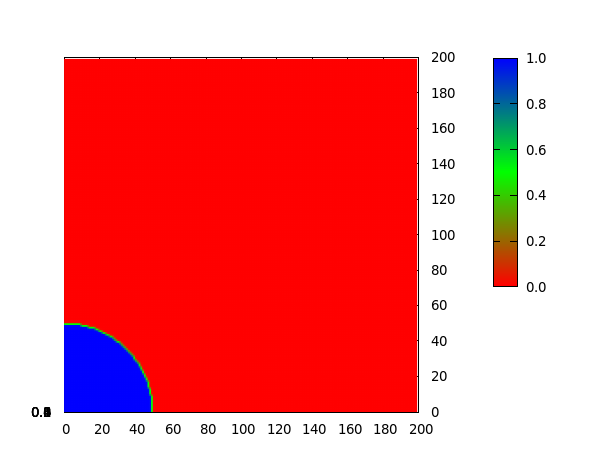
\includegraphics[width=.25\textwidth]{gt_0.png}
	\label{timestep 0}
	}
	\hspace{.25in}
	\subfloat[timestep 50000]{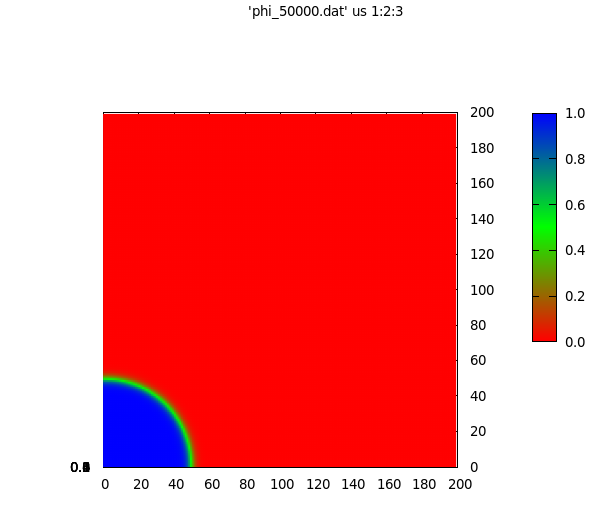
\includegraphics[width=.25\textwidth]{gt_50.png}
	\label{timestep 50000}
	}
	\hspace{.25in}
	\subfloat[timestep 150000]{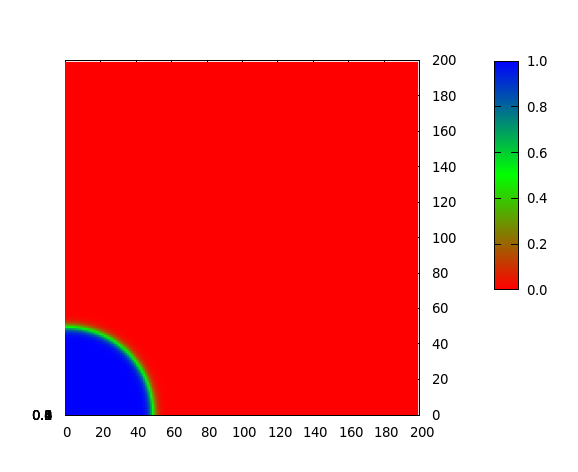
\includegraphics[width=.25\textwidth]{gt_99.png}
	\label{timestep 99000}
	}
	\centering
	\caption{Nuclei at critical radius - not growing}
	%\label{micros_3}
	\end{figure}
	
	\begin{figure}[!htbp]
	\centering
	\subfloat[timestep 0]{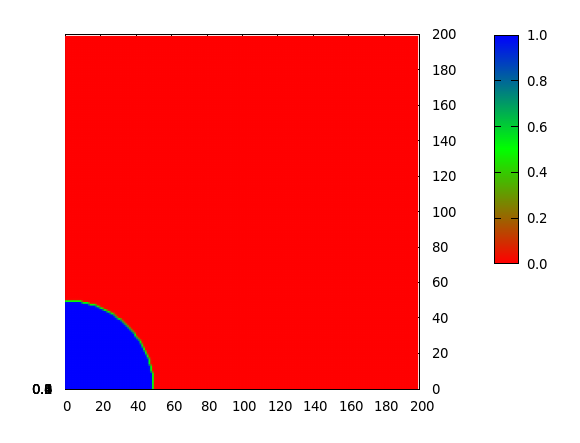
\includegraphics[width=.25\textwidth]{shrink_0.png}
	\label{timestep 0}
	}
	\hspace{.25in}
	\subfloat[timestep 50000]{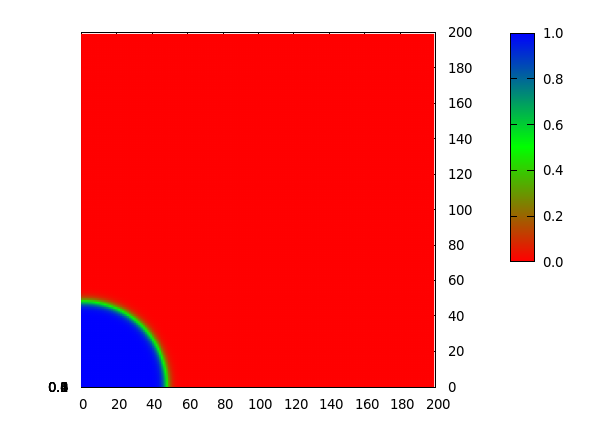
\includegraphics[width=.25\textwidth]{shrink_50.png}
	\label{timestep 50000}
	}
	\hspace{.25in}
	\subfloat[timestep 150000]{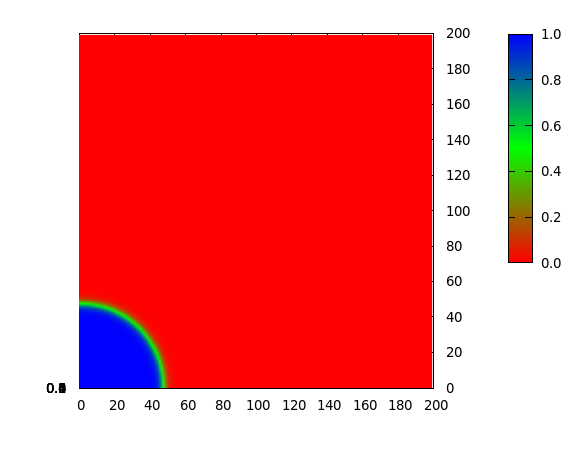
\includegraphics[width=.25\textwidth]{shrink_99.png}
	\label{timestep 99000}
	}
	\centering
	\caption{Nuclei Shrinking - $\mu$ less than critical}
	%\label{micros_3}
	\end{figure}
	
	\begin{figure}[!htbp]
	\centering
	\subfloat[timestep 0]{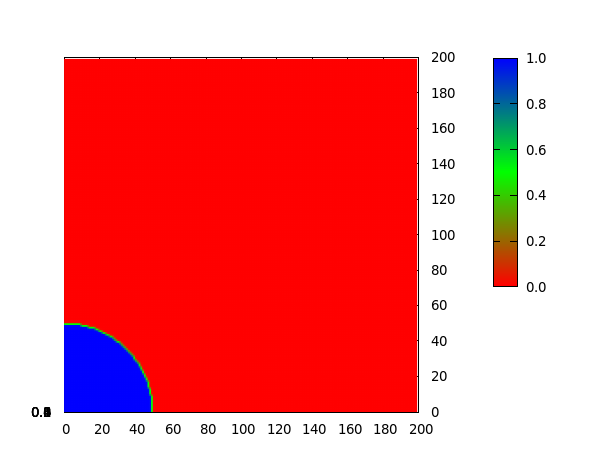
\includegraphics[width=.25\textwidth]{gt_0.png}
	\label{timestep 0}
	}
	\hspace{.25in}
	\subfloat[timestep 50000]{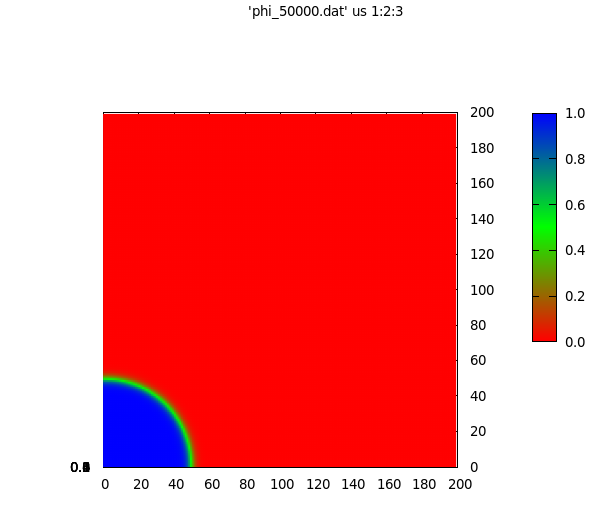
\includegraphics[width=.25\textwidth]{gt_50.png}
	\label{timestep 50000}
	}
	\hspace{.25in}
	\subfloat[timestep 99000]{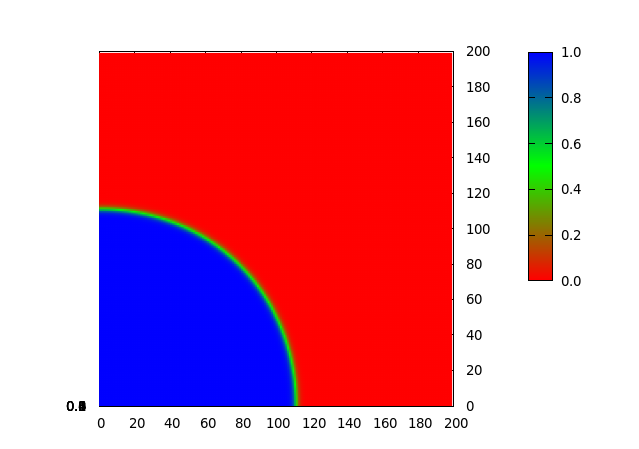
\includegraphics[width=.25\textwidth]{grow_99.png}
	\label{timestep 99000}
	}
	\centering
	\caption{Nuclei growing - $\mu$ greater than critical}
	%\label{micros_3}
	\end{figure}
	\newpage
	
	\subsection{Purturbation Analysis}
	The Mullins-Sekerka instability analysis gives a closed form
	analytical expression for sinusoidal purtubation of the plane
	front solution.\\
	\\
	The expression takes the following form;
	\begin{align*}
		\dfrac{\dot{\delta}}{\delta} &= V\tilde{\omega}\left[-\dfrac{b}{G} + \dfrac{1}{\tilde{\omega}}\left(k_{\omega} - \dfrac{V}{D}\right)\right]\\
		\text{where,  }
		\tilde{\omega} &= k_{\omega} - \dfrac{V}{D}(1-k)\\
		b &= \dfrac{\Gamma\omega^2}{\mu_{eq}(1-k)}\\
		\text{and   }
		k_{\omega} &= \dfrac{V}{2D} + \sqrt{\left(\dfrac{V}{2D}\right)^2 + \omega^2} 
	\end{align*}
	Where V is the velocity of the solidification front, D is 
	the solute diffusivity in the melt phase, $\Gamma$ is the 
	Gibbs Thompson coefficient, $\omega$ is the frequency of
	perturbation, $\delta$ is the amplitude of perturbation
	and $\dot{\delta}$ is the rate at which the amplitude is 
	changing.
	
	\begin{figure}[!htbp]
		\centering
		\subfloat[dispersion plot]{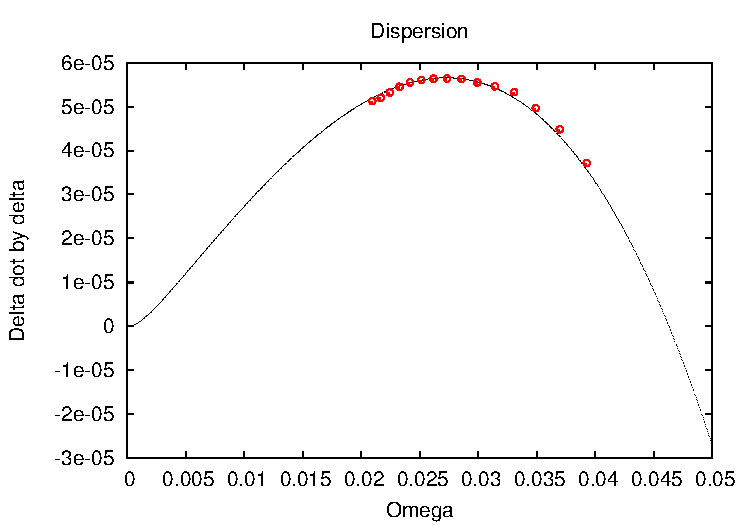
\includegraphics[width=.6\textwidth]{dispersion.pdf}
		\label{}
		}
		\hspace{.25in}
		\subfloat[sinusoidal $\phi$ front]{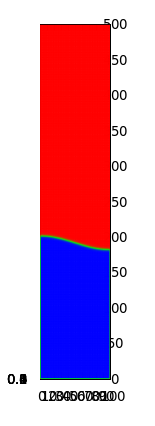
\includegraphics[width=.2\textwidth]{disp.png}
		\label{}
		}
	\end{figure}
	
\chapter{Results}
\section{One Dimensional Solidification Profile}

As a first test of the model, we tried to 
simulate solidification in one dimension for which the 
evoltuion profiles for state variables are well known. 
Mass transport is through diffusion only.
The evolving profiles of the phasefield vatiable, 
$\phi$, concentration and diffusion potential $\mu$ 
are depicted in the following images.

\begin{figure}[!htbp]
\centering
\subfloat[timestep 0]{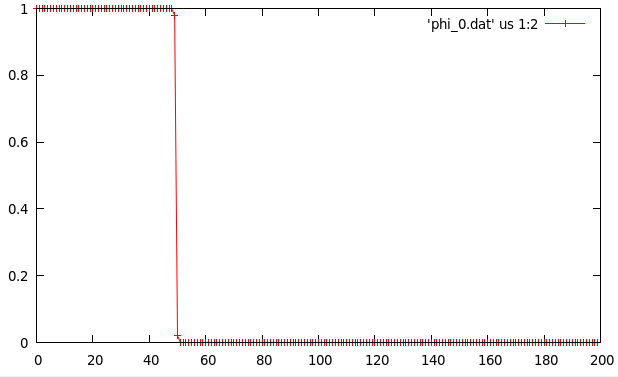
\includegraphics[width=.25\textwidth]{phi_0.png}
\label{timestep 0}}
\hspace{.25in}
\subfloat[timestep 50000]{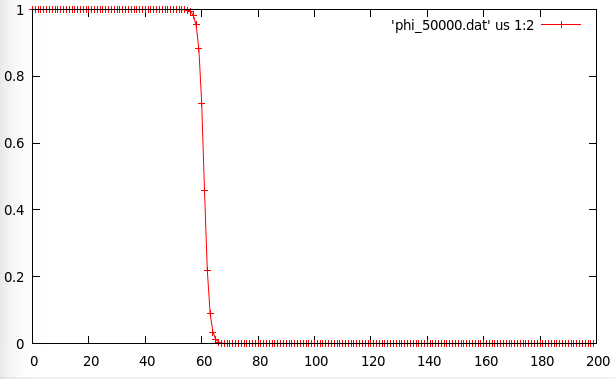
\includegraphics[width=.25\textwidth]{phi_50000.png}
\label{timestep 50000}
}
\hspace{.25in}
\subfloat[timestep 150000]{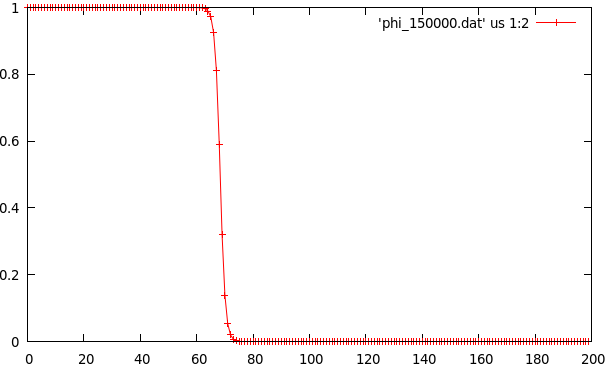
\includegraphics[width=.25\textwidth]{phi_150000.png}
\label{timestep 150000}
}
\centering
\caption{time evolution of the phase field variable $\phi$}
%\label{micros_3}
\end{figure}
 
\begin{figure}[!htbp]
\centering
\subfloat[timestep 0]{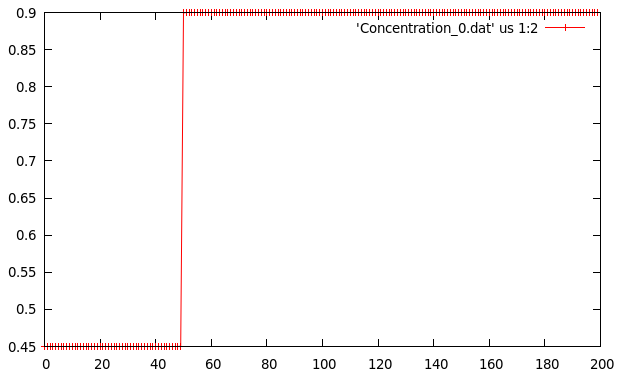
\includegraphics[width=.25\textwidth]{conc_0.png}
\label{timestep 0}
}
\hspace{.25in}
\subfloat[timestep 50000]{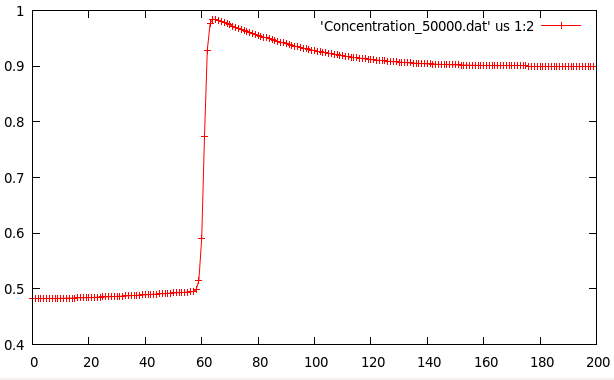
\includegraphics[width=.25\textwidth]{conc_50000.png}
\label{timestep 50000}
}
\hspace{.25in}
\subfloat[timestep 150000]{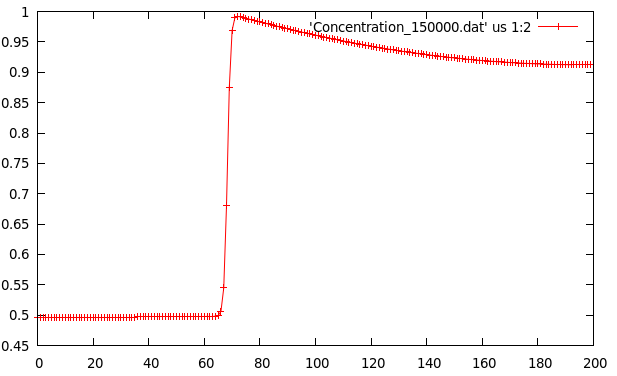
\includegraphics[width=.25\textwidth]{conc_150000.png}
\label{timestep 150000}
}
\centering
\caption{time evolution of concentration}
%\label{micros_3}
\end{figure}

\begin{figure}[!htbp]
\centering
\subfloat[timestep 0]{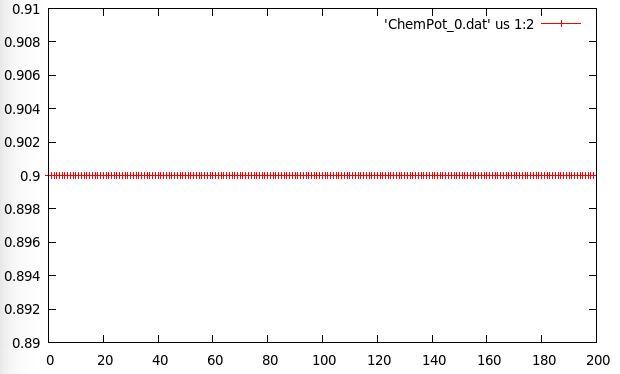
\includegraphics[width=.25\textwidth]{chem_0.png}
\label{timestep 0}
}
\hspace{.25in}
\subfloat[timestep 50000]{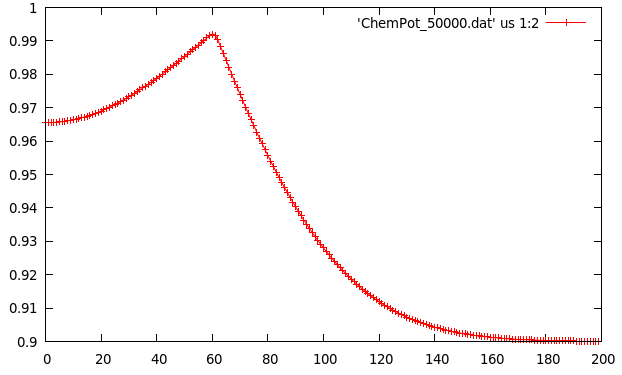
\includegraphics[width=.25\textwidth]{chem_50000.png}
\label{timestep 50000}
}
\hspace{.25in}
\subfloat[timestep 150000]{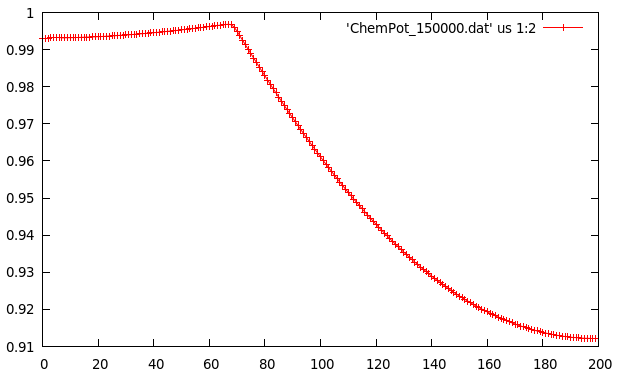
\includegraphics[width=.25\textwidth]{chem_150000.png}
\label{timestep 150000}
}
\centering
\caption{time evolution of chemical potential $\mu$}
%\label{micros_3}
\end{figure}
\newpage

\section{Anisotropic Solidification in 2D - only diffusion}
Following images depict the $\phi$ profile during anisotropic 
solidification at different time steps. 
\begin{figure}[!h]
\centering
\subfloat[timestep 0]{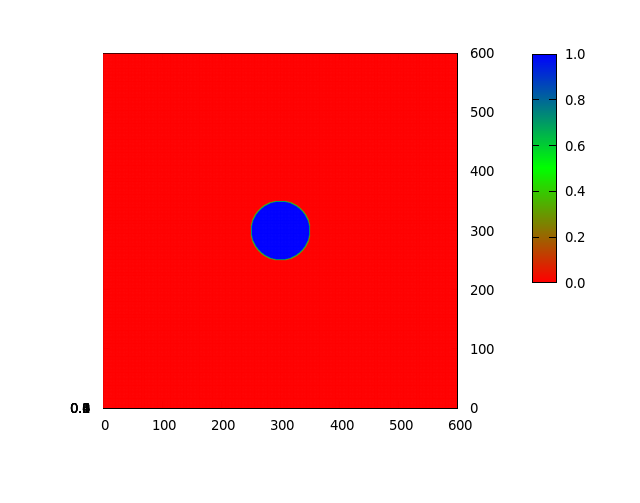
\includegraphics[width=.25\textwidth]{dendrite_0.png}
\label{timestep 0}
}
\hspace{.25in}
\subfloat[timestep 15000]{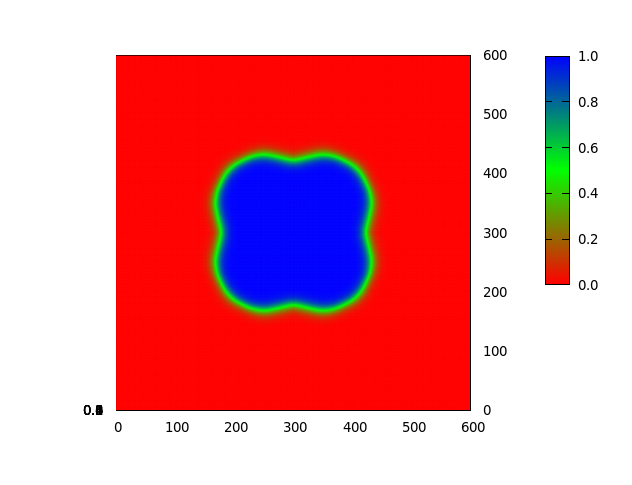
\includegraphics[width=.25\textwidth]{dendrite_15000.png}
\label{timestep 50000}
}
\hspace{.25in}
\subfloat[timestep 30000]{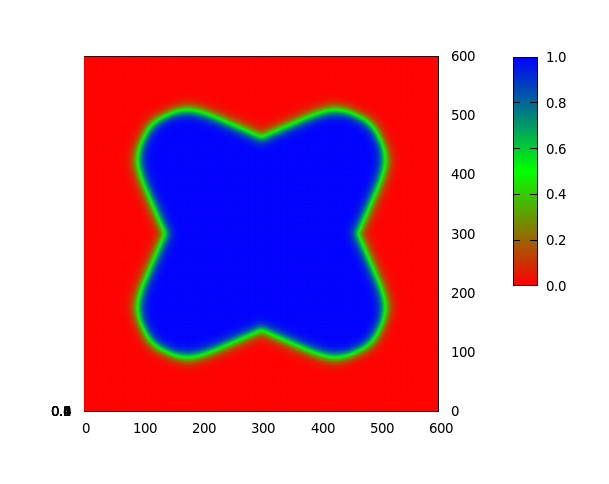
\includegraphics[width=.25\textwidth]{dendrite_30000.png}
\label{timestep 99000}
}
\centering
\caption{Dendritic solidification on introducing anisotropy}
%\label{micros_3}
\end{figure}

\section{Phasefield - Navier Stokes}
	
	\subsection*{Poiseuille flow}
	
	\begin{figure}[!htbp]
	\centering
	\subfloat[timestep 1000]{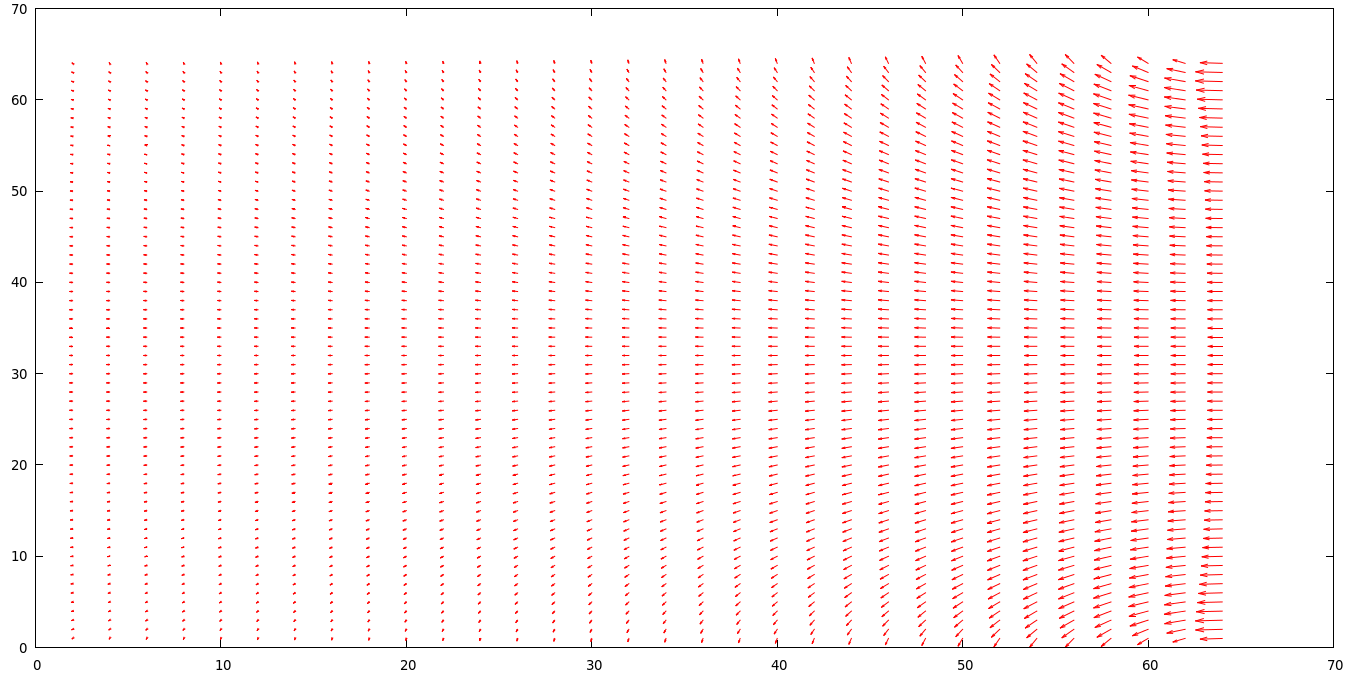
\includegraphics[width=.25\textwidth]{pflow_1000.png}
	%\label{timestep 0}
	}
	\hspace{.25in}
	\subfloat[timestep 10000]{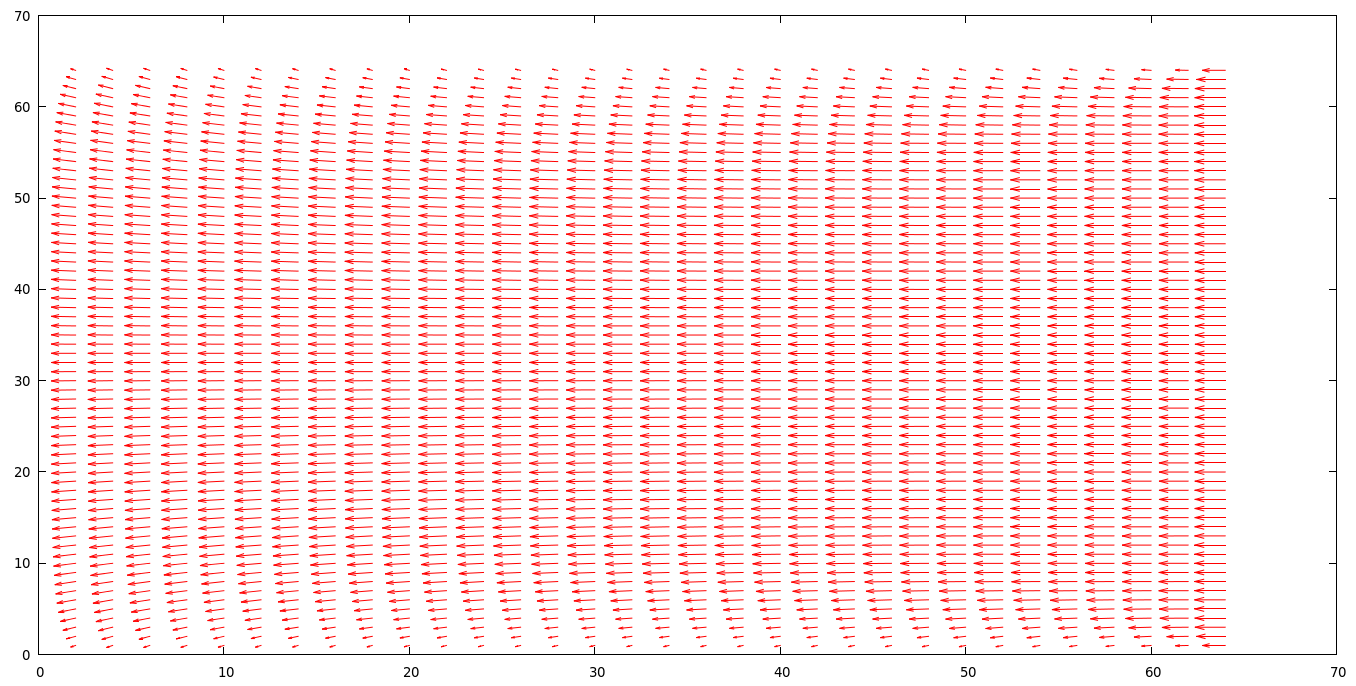
\includegraphics[width=.25\textwidth]{pflow_10000.png}
	%\label{timestep 50000}
	}
	\hspace{.25in}
	\subfloat[timestep 50000]{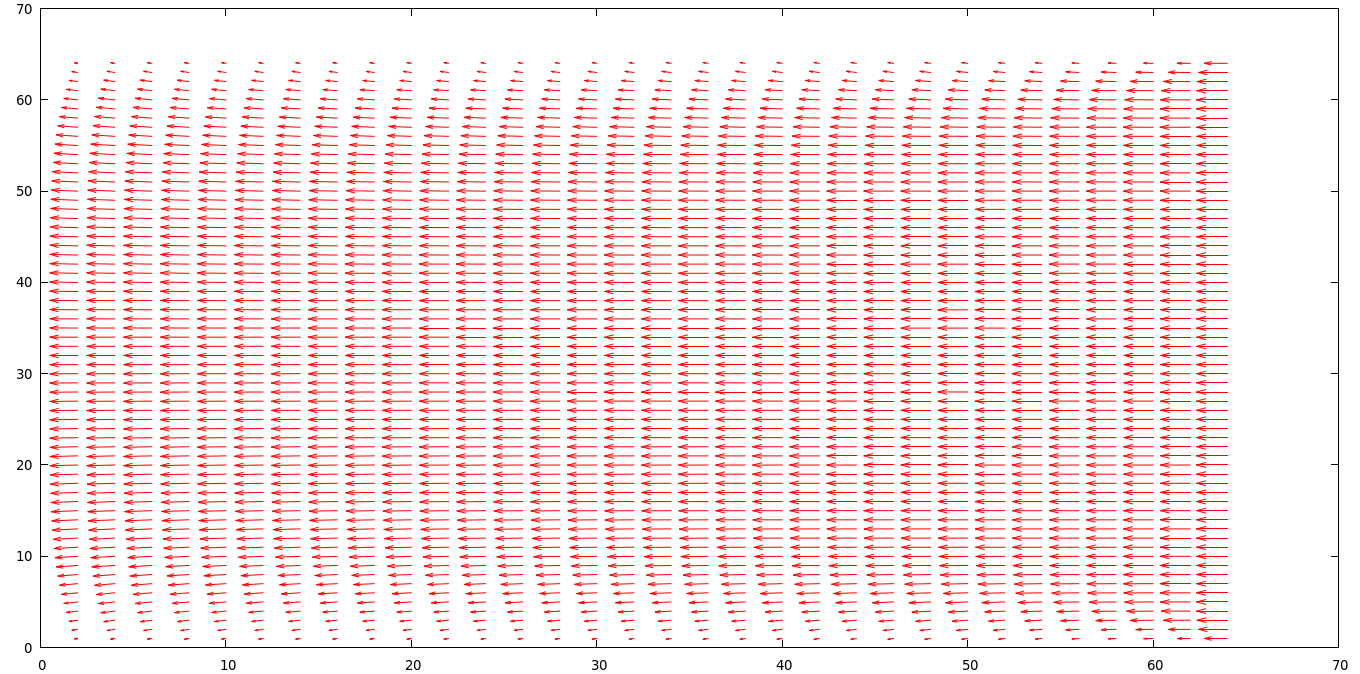
\includegraphics[width=.25\textwidth]{pflow_50000.png}
	%\label{timestep 50000}
	}
	\centering
	\caption{Pressure difference between East and West walls}
	\end{figure}
	
	\subsection*{Flow around a solid object in a closed space}
	
	\begin{figure}[h]
	\centering
	\subfloat[timestep 1000]{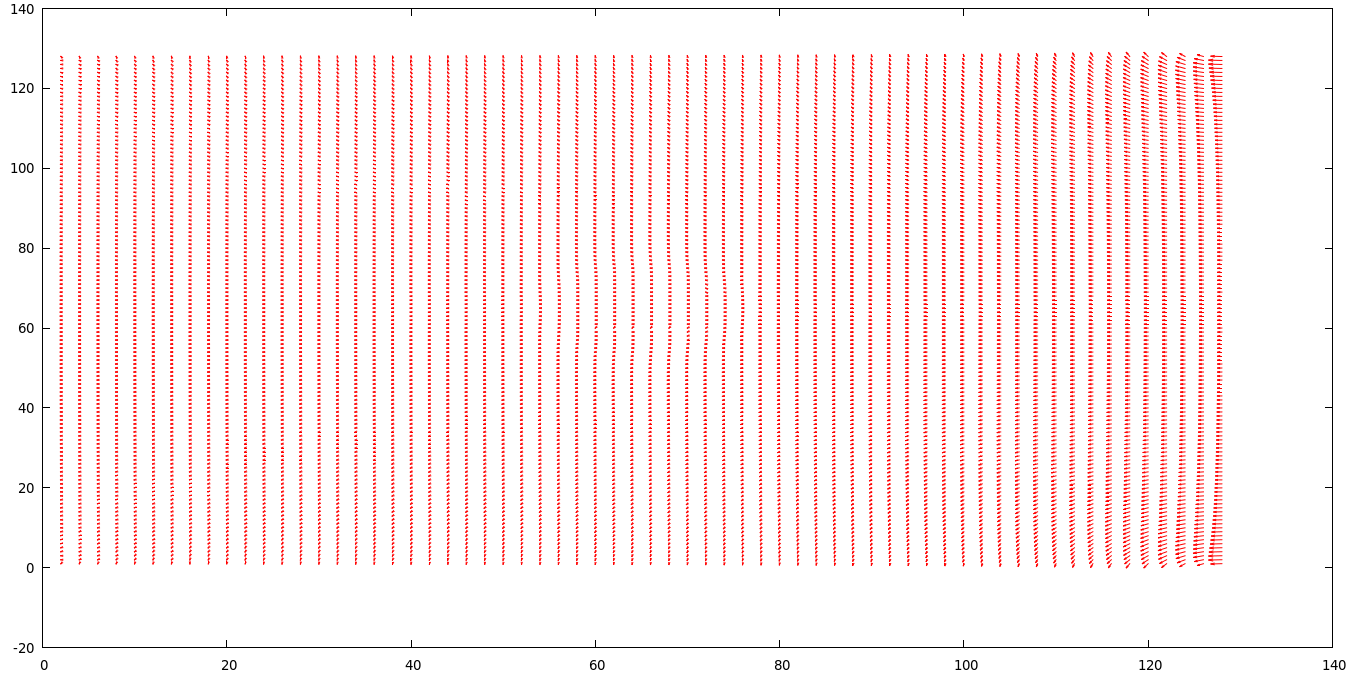
\includegraphics[width=.25\textwidth]{object_1000.png}
	%\label{timestep 0}
	}
	\hspace{.25in}
	\subfloat[timestep 10000]{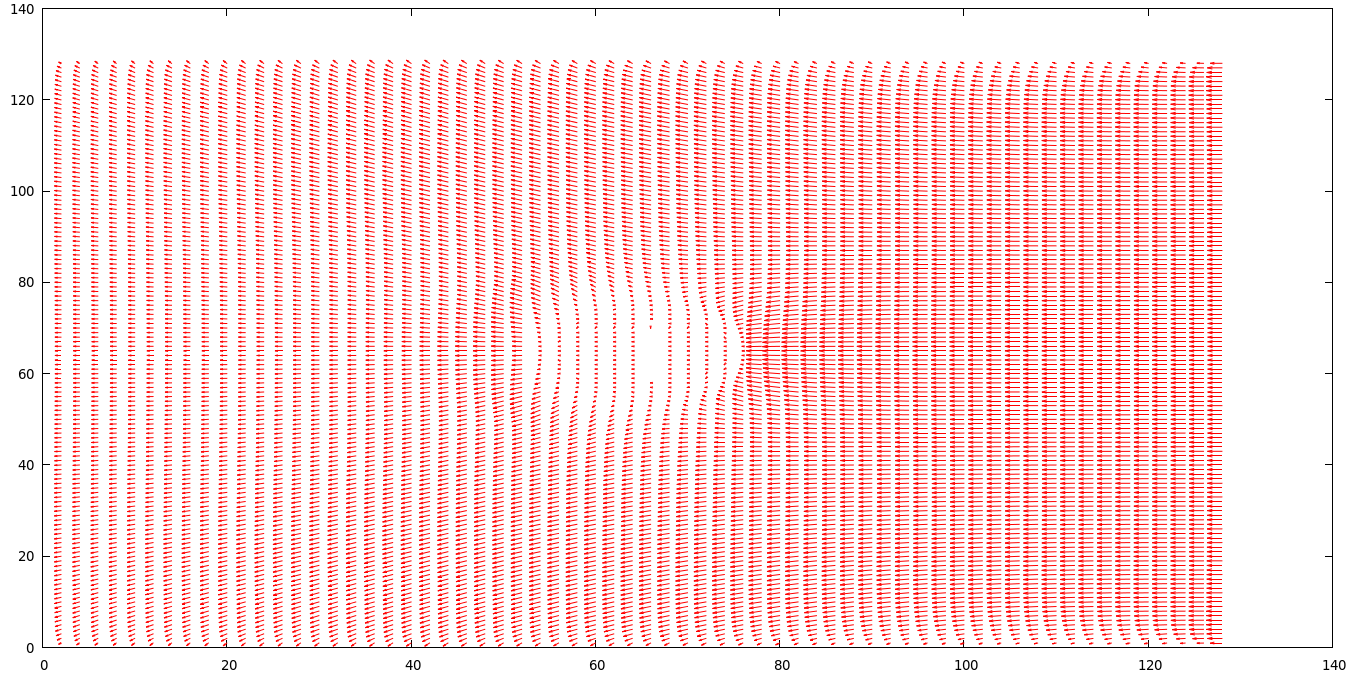
\includegraphics[width=.25\textwidth]{object_10000.png}
	%\label{timestep 50000}
	}
	\hspace{.25in}
	\subfloat[timestep 50000]{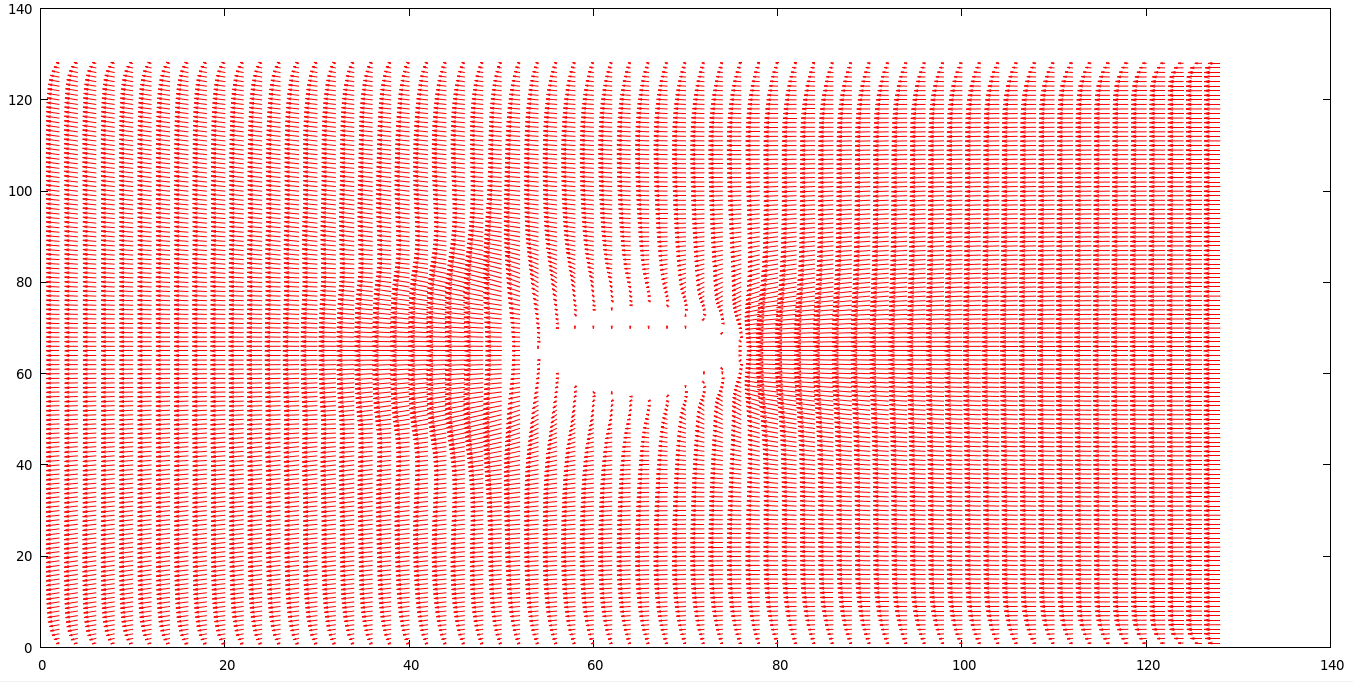
\includegraphics[width=.25\textwidth]{object_50000.png}
	%\label{timestep 50000}
	}
	\centering
	\caption{Flow around a solid with a diffuse interface}
	\end{figure}
	\newpage
	\subsection*{Anisotropic growth during fluid flow}
	Following images depict the evolution of the flow profile 
	[left to right] and the solid phase over time.
			\begin{figure}[H]
				\centering
				\subfloat[timestep 20000]{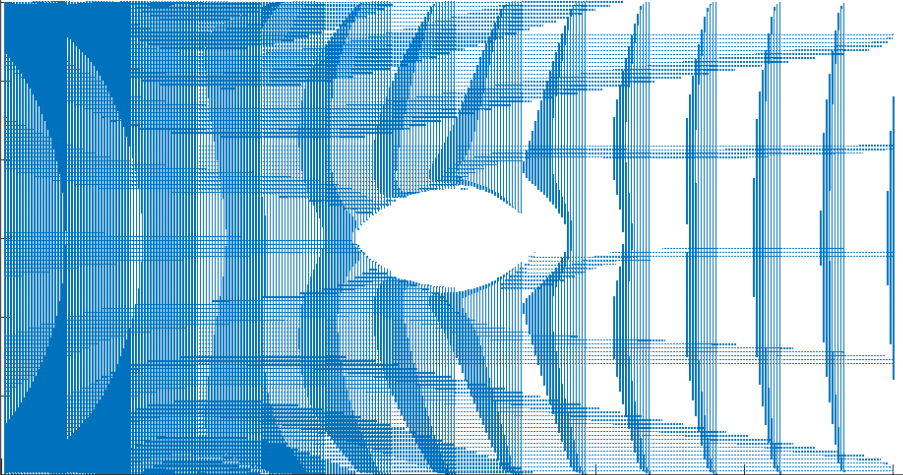
\includegraphics[width=.3\textwidth]{20k.png}
				}
				\hspace{.25in}
				\subfloat[timestep 65000]{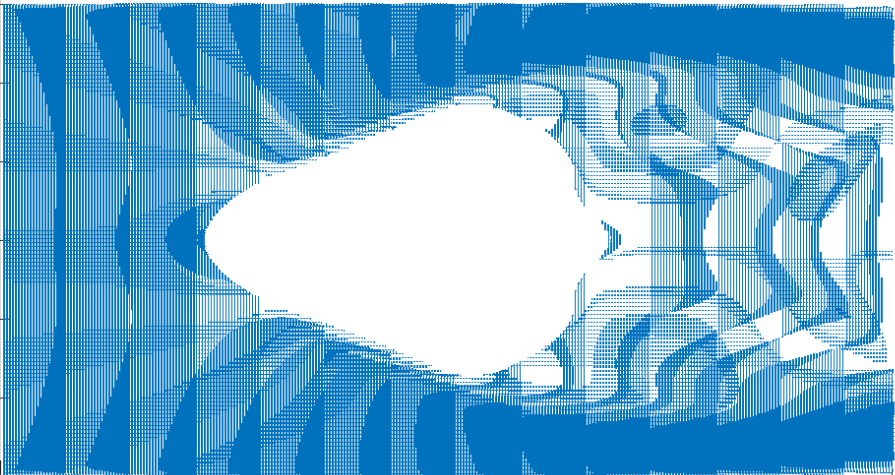
\includegraphics[width=.3\textwidth]{65k.png}
				}
				\centering
				\caption{Forced Covection; left to right around evolving solid phase}
			\end{figure}
			\begin{figure}[!h]
				\centering
				\subfloat[timestep 20000]{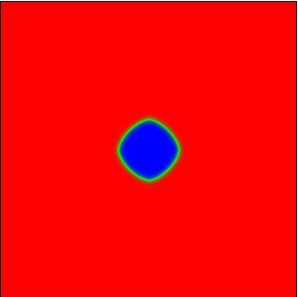
\includegraphics[width=.3\textwidth]{phi_20k.png}}
				\hspace{.25in}
				\subfloat[timestep 65000]{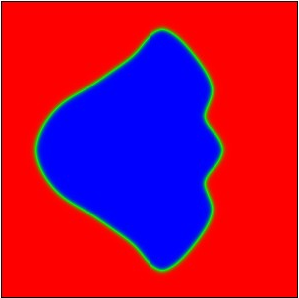
\includegraphics[width=.3\textwidth]{phi_65k.png}}
				\centering
				\caption{Evolving solid phase}
			\end{figure}
\newpage
\section{Phasefield - Lattice Boltzmann}
Having incorporated the lattice-Boltzmann based flow solver described earlier into
our phasefield solver for solidification, we validated the solver by simulating 
the lid driven cavity flow and got expected results as seen in figure a.\\
\\
Thereafter, we simulated anisotropic growth in presence of forced pipe flow 
[left to right] resulting in $\mu$ profiles as seen in figure b and figure c. 
					\begin{figure}[H]
						\centering
						\subfloat[lid driven cavity]{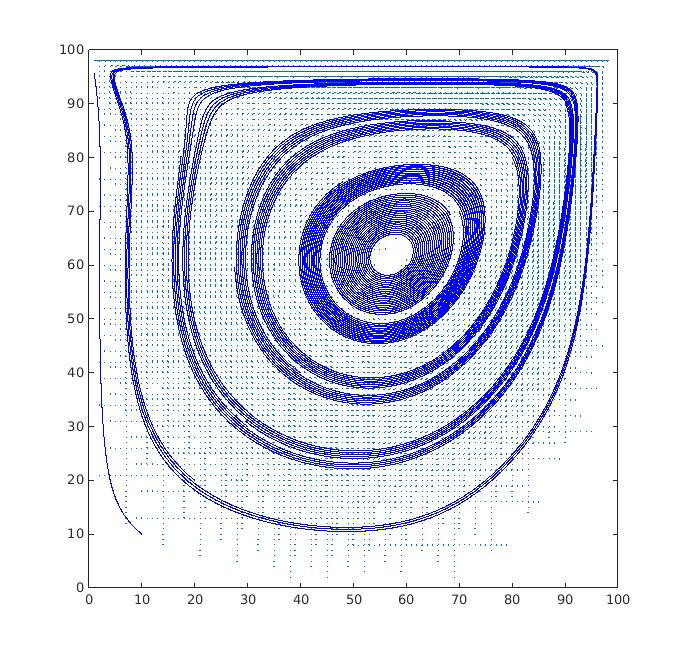
\includegraphics[width=.3\textwidth]{lbm_100_11k.jpg}
						\label{lid driven cavity}
						}
						\hspace{.3in}
						\subfloat[mu field]{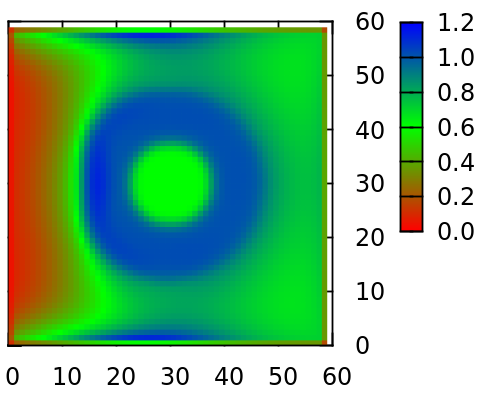
\includegraphics[width=.3\textwidth]{mu_3k.png}
						\label{}
						}
						\hspace{.3in}
						\subfloat[mu field]{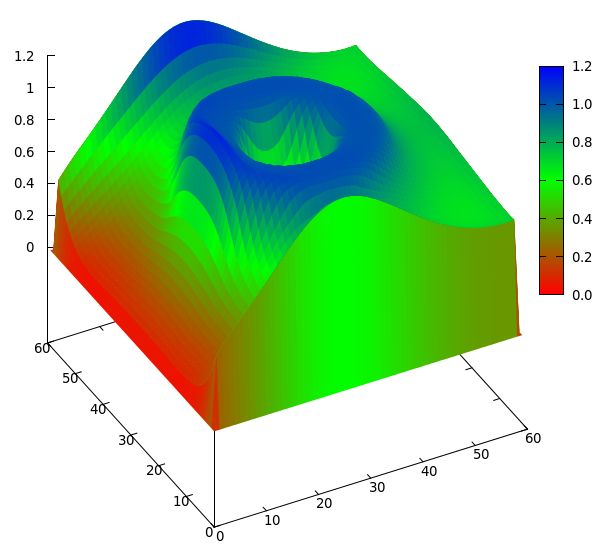
\includegraphics[width=.3\textwidth]{mu_3k_3d.png}
						\label{}
						}
						\centering
						\caption{Examples of flow profiles generated using lbm}
						%\label{micros_3}
					\end{figure}

\begin{thebibliography}{1}
	
  \bibitem{MS_theory} J.S. Langer, in Chance and Matter edited by J. Souletie, J. Vannenimus 
	and R Stora (North Holland, Amsterdam 1987), p. 629; D Kessler, J Koplik and H Levine, Adv. 
	Phys. 37, 255 (1988); E .A. Brenner and V.I. Mel'nikov, \textit{ibid}. 40, 53 (1991)
	
  \bibitem{langer} J. S. Langer, Phys. Rev. Lett., Volume 44, Number 15, 14 April 1980 

  \bibitem{Stein} I. Steinbach, Acta Materialia 57 (2009) 2640 - 2645

  \bibitem{Tong} Tong et al., Phys. Rev. E, vol. 61, No. 1, January 2000

  \bibitem{Abhik_1} Abhik Chaudhary and Britta Nestler, Phys. Rev. E 85,021602 (2012)
  
  \bibitem{Abhik_2} Britta Nestler and Abhik Chaudhary, Current Opinion in solid State 
  and Materials Science 15(2011) 93-105
  
  \bibitem{Beck} C. Beckermann et al., Jour. of Comp. Phys. 154, 468-496 (1999)
  
  \bibitem{Boet} W.J. Boettinger el al., Annu. Rev. Mater. Res. 2002. 32:163-94
  
  \bibitem{l_1} Yuanxun Bill Bao \& Justin Meskas, "Lattice Boltzmann Model for Fluid Simulations", April 14, 2011
  
  \bibitem{l_2} Igor Mele, "Lattice Boltzmann method", March 2013 
  
  \bibitem{l_3} Zou \& He, "On pressure and velocity boundary conditions for the lattice Boltzmann BGK model", {\em Phys. Fluids}, {\bf 9}(6), June 1997 
  
  \bibitem{l_4} Britta Nestler, Ali Aksi, Michael Selzer, "Combined lattice Boltzmann and phase-field simulations for incompressible fluid flow in porous media", {\em Mathematics and Computers in Simulation}, 80(2010) 1458-1468
	
\end{thebibliography}
\end{document}